\chapter{Integration}
\setcounter{section}{11}
\setcounter{subsection}{0}
\setcounter{subsubsection}{1}
\setcounter{secnumdepth}{4}
\subsection{Integration}
\href{https://youtu.be/MOoeV2ewtj8}{Video 01}\\
\begin{center}
	
	Sei $ f:[a,b] \longmapsto \mathbb{R}$
	
	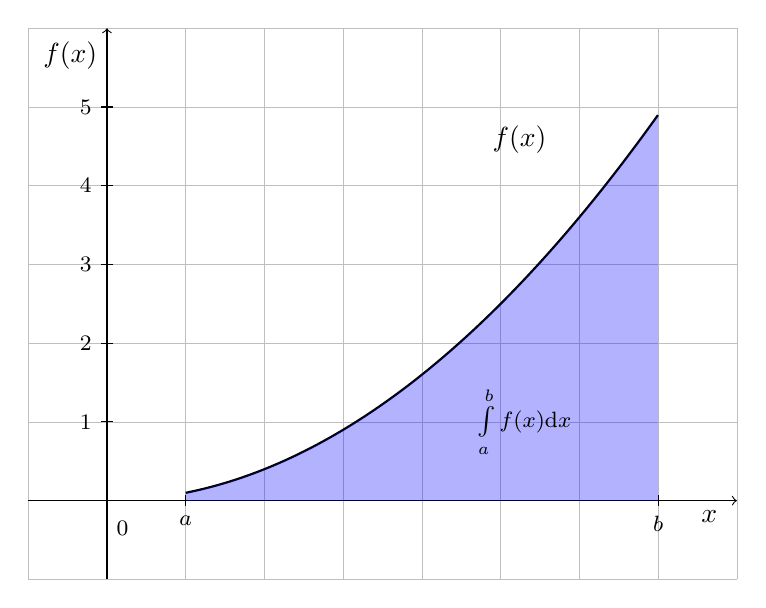
\begin{tikzpicture}[xscale=1, yscale=1]
	
	% Gitternetzlinien
	\draw[xstep=1cm, ystep=1cm, very thin, color=lightgray] (-1,6) grid (8,-1);
	% x-Achse
	\draw[->] (-1,0) -- (8,0) node[below,xshift=-1em] {$x$}; 
	%Zahlen auf x-Achse
	%\foreach \x in {-3,...,-1}
	%\draw[shift={(\x,0)},color=black] (0pt,2pt) -- (0pt,-2pt) node[below] {\footnotesize $\x$};
	%\foreach \x in {a,...,7}
	%\draw[shift={(\x,0)},color=black] (0pt,2pt) -- (0pt,-2pt) node[below] {\footnotesize $\x$};
	
	% y-Achse 
	\draw[->] (0,-1) -- (0,6) node[left,yshift=-1em] {$f(x)$};%node[above left]
	%Zahlen auf y-Achse
	%\foreach \y in {-1,...,-1}
	%\draw[shift={(0,\y)},color=black] (2pt,0pt) -- (-2pt,0pt) node[left] {\footnotesize $\y$};
	\foreach \y in {1,...,5}
	\draw[shift={(0,\y)},color=black] (2pt,0pt) -- (-2pt,0pt) node[left] {\footnotesize $\y$};
	%Ursprung
	\draw[color=black] (0pt,-10pt) node[right] {\footnotesize $0$};
	
	\draw[thick,color=black] plot[samples=200, domain=1:7] 
	(\x,{0.1*\x^2}) node[below, xshift=-5em] {$f(x)$};
	
	\fill[color =blue,fill opacity=0.3] plot[domain=1:7] (\x,{(0.1*\x^2 })% 
	-- plot[domain=7:1] (\x,{0});% 
	
	\draw[shift={(1,0)},color=black] (0pt,2pt) -- (0pt,-2pt) node[below] {\footnotesize $a$};
	\draw[shift={(7,0)},color=black] (0pt,2pt) -- (0pt,-2pt) node[below] {\footnotesize $b$};
	\draw[color=black] (5.3,1) node {\footnotesize $\int\limits_{a}^{b} f(x)\mathrm{d}x$};
	\end{tikzpicture}\\
\end{center}
Das bestimmte Integral $\int\limits_{a}^{b} f(x)\mathrm{d}x  $ ist die orientierte Fläche zwischen $ a,b $, die zwischen $ f(x) $ und der x-Achse ist. Oberhalb der x-Achse ist die Fläche positiv und unterhalb negativ.\\
\pagebreak

Durch Zerlegung von $ [a,b] $ in gleichgroße Teile kann man die Flächen berechnen.\\
\begin{center}
	$ a=x_0<x_1<x_3\ldots<x_n=3 $\\
	
	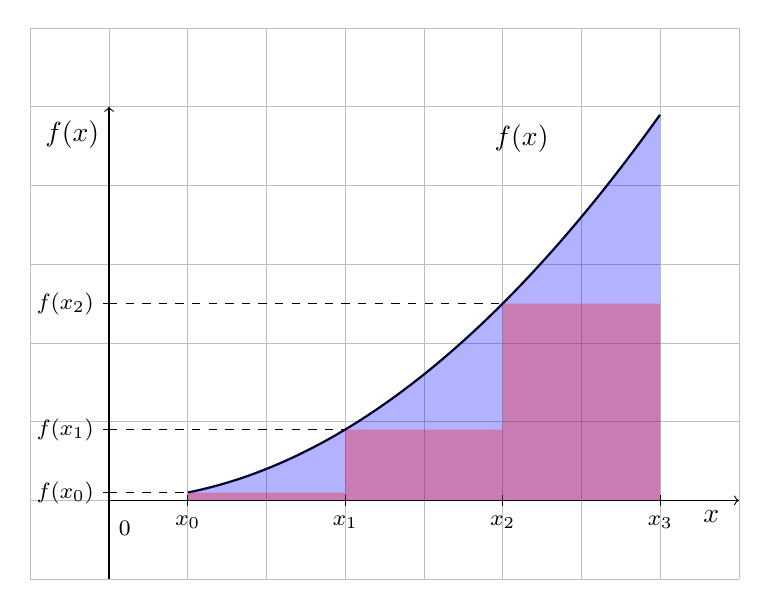
\begin{tikzpicture}[xscale=1, yscale=1]
	
	% Gitternetzlinien
	\draw[xstep=1cm, ystep=1cm, very thin, color=lightgray] (-1,6) grid (8,-1);
	% x-Achse
	\draw[->] (0,0) -- (8,0) node[below,xshift=-1em] {$x$}; 
	%Zahlen auf x-Achse
	%\foreach \x in {-3,...,-1}
	%\draw[shift={(\x,0)},color=black] (0pt,2pt) -- (0pt,-2pt) node[below] {\footnotesize $\x$};
	%\foreach \x in {a,...,7}
	%\draw[shift={(\x,0)},color=black] (0pt,2pt) -- (0pt,-2pt) node[below] {\footnotesize $\x$};
	
	% y-Achse 
	\draw[->] (0,-1) -- (0,5) node[left,yshift=-1em] {$f(x)$};%node[above left]
	%Zahlen auf y-Achse
	%\foreach \y in {-1,...,-1}
	%\draw[shift={(0,\y)},color=black] (2pt,0pt) -- (-2pt,0pt) node[left] {\footnotesize $\y$};
	%\foreach \y in {1,...,5}
	%\draw[shift={(0,\y)},color=black] (2pt,0pt) -- (-2pt,0pt) node[left] {\footnotesize $\y$};
	\draw[shift={(0,0.1)},color=black] (2pt,0pt) -- (-2pt,0pt) node[left] {\footnotesize $f(x_0)$};
	\draw[color=black,dashed] (0,0.1)--(1,0.1);
	\draw[shift={(0,0.9)},color=black] (2pt,0pt) -- (-2pt,0pt) node[left] {\footnotesize $f(x_1)$};
	\draw[color=black,dashed] (0,0.9)--(3,0.9);
	\draw[shift={(0,2.5)},color=black] (2pt,0pt) -- (-2pt,0pt) node[left] {\footnotesize $f(x_2)$};
	\draw[color=black,dashed] (0,2.5)--(5,2.5);
	
	%Ursprung
	\draw[color=black] (0pt,-10pt) node[right] {\footnotesize $0$};
	
	\draw[thick,color=black] plot[samples=200, domain=1:7] 
	(\x,{0.1*\x^2}) node[below, xshift=-5em] {$f(x)$};
	
	\fill[color =blue,fill opacity=0.3] plot[domain=1:7] (\x,{(0.1*\x^2 })% 
	-- plot[domain=7:1] (\x,{0});% 
	\draw[shift={(5,0)},color=black] (0pt,2pt) -- (0pt,-2pt) node[below] {\footnotesize $x_2$};
	\draw[shift={(3,0)},color=black] (0pt,2pt) -- (0pt,-2pt) node[below] {\footnotesize $x_1$};
	\draw[shift={(1,0)},color=black] (0pt,2pt) -- (0pt,-2pt) node[below] {\footnotesize $x_0$};
	\draw[shift={(7,0)},color=black] (0pt,2pt) -- (0pt,-2pt) node[below] {\footnotesize $x_3$};
	%\draw[color=black] (5.3,1) node {A};
	%\draw[color=red] (1,0) -- (3,0)--(3,0.1)--(1,0.1)--(1,0);
	%\draw[color=red] (3,0) -- (5,0)--(5,0.9)--(3,0.9)--(3,0);
	%\draw[color=red] (5,0) -- (7,0)--(7,2.5)--(5,2.5)--(5,0);
	\fill[color =red,fill opacity=0.3] plot[domain=1:3] (\x,{(0.1 })% 
	-- plot[domain=3:1] (\x,{0});% 
	\fill[color =red,fill opacity=0.3] plot[domain=3:5] (\x,{(0.9 })% 
	-- plot[domain=5:3] (\x,{0});% 
	\fill[color =red,fill opacity=0.3] plot[domain=5:7] (\x,{(2.5 })% 
	-- plot[domain=7:5] (\x,{0});% 
	\end{tikzpicture}\\	
	
\end{center}
Die Fläche unter der Funktion $ f(x) $ ist dannn die Summe von A:\\
\begin{center}
	
	
	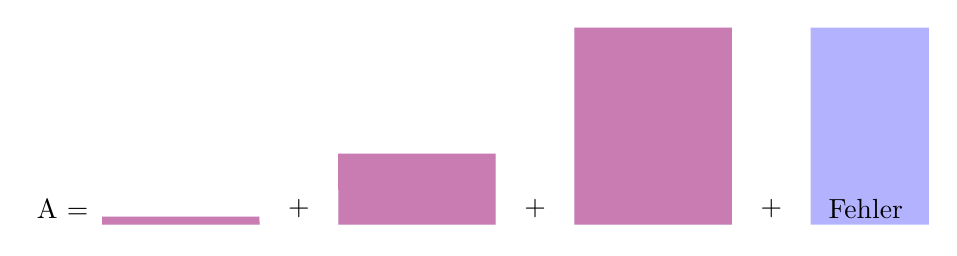
\begin{tikzpicture}[xscale=1, yscale=1]
	\draw[color=black] (0.5,0.2) node {A =};
	\draw[color=black] (3.5,0.2) node {+};
	\draw[color=black] (6.5,0.2) node {+};
	\draw[color=black] (9.5,0.2) node {+};
	%\draw[color=red] (1,0) -- (3,0)--(3,0.1)--(1,0.1)--(1,0);
	%\draw[color=red] (4,0) -- (6,0)--(6,0.9)--(4,0.9)--(4,0);
	%\draw[color=red] (7,0) -- (9,0)--(9,2.5)--(7,2.5)--(7,0);
	\fill[color =blue,fill opacity=0.3] plot[domain=1:3] (\x,{(0.1 })% 
	-- plot[domain=3:1] (\x,{0});% 
	\fill[color =blue,fill opacity=0.3] plot[domain=4:6] (\x,{(0.9 })% 
	-- plot[domain=6:4] (\x,{0});% 
	\fill[color =blue,fill opacity=0.3] plot[domain=7:9] (\x,{(2.5 })% 
	-- plot[domain=9:7] (\x,{0});% 
	
	\fill[color =red,fill opacity=0.3] plot[domain=1:3] (\x,{(0.1 })% 
	-- plot[domain=3:1] (\x,{0});% 
	\fill[color =red,fill opacity=0.3] plot[domain=4:6] (\x,{(0.9 })% 
	-- plot[domain=6:4] (\x,{0});% 
	\fill[color =red,fill opacity=0.3] plot[domain=7:9] (\x,{(2.5 })% 
	-- plot[domain=9:7] (\x,{0});% 
	\fill[color =blue,fill opacity=0.3] plot[domain=10:11.5] (\x,{(2.5 })% 
	-- plot[domain=11.5:10] (\x,{0});% 
	\draw[color=black] (10.7,0.2) node {Fehler};
	\end{tikzpicture}\\
\end{center}
\begin{align*}
\mathrm{A}=f(x_0)\cdot (x_1-x_0)+f(x_1)\cdot (x_2-x_1)+f(x_2)\cdot (x_3-x_2)+\mathrm{Fehler}
\end{align*}
Bei Verwendung von viele Flächen wird der Fehler immer kleiner.\\
\begin{center}
	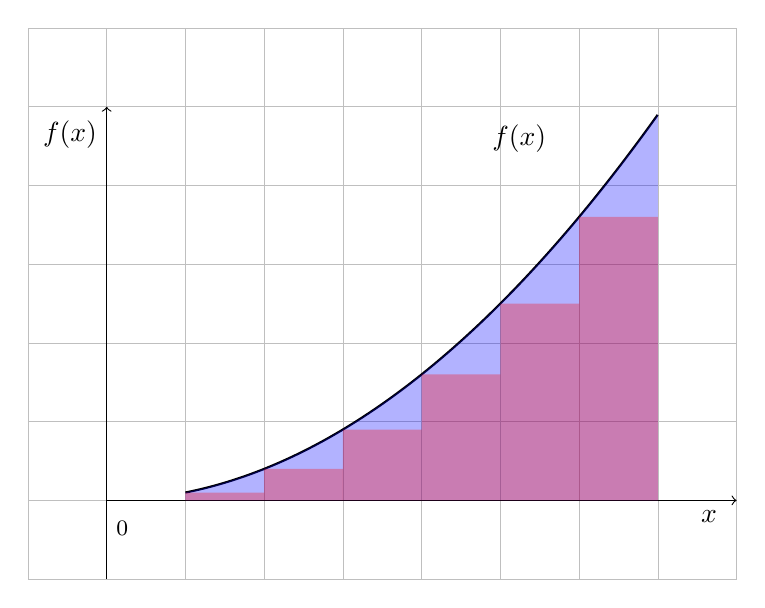
\begin{tikzpicture}[xscale=1, yscale=1]
	
	% Gitternetzlinien
	\draw[xstep=1cm, ystep=1cm, very thin, color=lightgray] (-1,6) grid (8,-1);
	% x-Achse
	\draw[->] (0,0) -- (8,0) node[below,xshift=-1em] {$x$}; 
	%Zahlen auf x-Achse
	%\foreach \x in {-3,...,-1}
	%\draw[shift={(\x,0)},color=black] (0pt,2pt) -- (0pt,-2pt) node[below] {\footnotesize $\x$};
	%\foreach \x in {a,...,7}
	%\draw[shift={(\x,0)},color=black] (0pt,2pt) -- (0pt,-2pt) node[below] {\footnotesize $\x$};
	
	% y-Achse 
	\draw[->] (0,-1) -- (0,5) node[left,yshift=-1em] {$f(x)$};%node[above left]
	%Zahlen auf y-Achse
	%\foreach \y in {-1,...,-1}
	%\draw[shift={(0,\y)},color=black] (2pt,0pt) -- (-2pt,0pt) node[left] {\footnotesize $\y$};
	%\foreach \y in {1,...,5}
	%\draw[shift={(0,\y)},color=black] (2pt,0pt) -- (-2pt,0pt) node[left] {\footnotesize $\y$};
	
	
	%Ursprung
	\draw[color=black] (0pt,-10pt) node[right] {\footnotesize $0$};
	
	\draw[thick,color=black] plot[samples=200, domain=1:7] 
	(\x,{0.1*\x^2}) node[below, xshift=-5em] {$f(x)$};
	
	\fill[color =blue,fill opacity=0.3] plot[domain=1:7] (\x,{(0.1*\x^2 })% 
	-- plot[domain=7:1] (\x,{0});% 
	
	
	\fill[color =red,fill opacity=0.3] plot[domain=1:2] (\x,{(0.1 })% 
	-- plot[domain=2:1] (\x,{0});% 
	\fill[color =red,fill opacity=0.3] plot[domain=2:3] (\x,{(0.4 })% 
	-- plot[domain=3:2] (\x,{0});% 
	\fill[color =red,fill opacity=0.3] plot[domain=3:4] (\x,{(0.9 })% 
	-- plot[domain=4:3] (\x,{0});% 
	\fill[color =red,fill opacity=0.3] plot[domain=4:5] (\x,{(1.6 })% 
	-- plot[domain=5:4] (\x,{0});% 
	\fill[color =red,fill opacity=0.3] plot[domain=5:6] (\x,{(2.5 })% 
	-- plot[domain=6:5] (\x,{0});% 
	\fill[color =red,fill opacity=0.3] plot[domain=6:7] (\x,{(3.6 })% 
	-- plot[domain=7:6] (\x,{0});% 
	\end{tikzpicture}\\	
	
\end{center}
Bei $ n- $Flächen gilt dann allgemein:\\
\begin{align*}
\mathrm{A}&=f(x_0)(x_1-x_0)+f(x_1)(x_2-x_1)+\ldots +f(x_{x_{n-1}})(x_n-x_{x_{n-1}})+\mathrm{Fehler}(n)\\
&=\sum\limits_{k=1}^{n}f(x_{x_{k-1}})(x_k-x_{x_{k-1}})+\mathrm{Fehler}(n)\\
\end{align*}
Man definiert:\\
\begin{align*}
\Delta_{x_k}=(x_k-x_{k-1})
\end{align*}
Dann gilt für die Summe: $ \mathrm{S}_n $\\
\begin{align*}
\mathrm{S}_n=\mathrm{A}=\sum\limits_{k=1}^{n}f(x_{k-1})\Delta_{x_k}+\mathrm{Fehler}(n)
\end{align*}
Dadurch, dass man die Summentteile unendlich klein wählt wird der Fehler Null, dann gilt für $ n\rightarrow\infty $ das bestimmte Integral:\\
\begin{align*}
\int\limits_{a}^{b} f(x)\mathrm{d}x=\lim\limits_ {n\to\infty} \mathrm{S}_n
\end{align*}
Ist die Funktion $ f:[a,b] \longmapsto \mathbb{R}$ monoton oder stetig dann existiert:\\
\begin{align*}
\lim\limits_ {n\to\infty} \mathrm{S}_n=\int\limits_{a}^{b} f(x)\mathrm{d}x
\end{align*}
Beispiel:\\
(i) $ f:[0,1] \longmapsto \mathbb{R} $ mit $ x\longmapsto 1 $\\
\begin{center}
	
	
	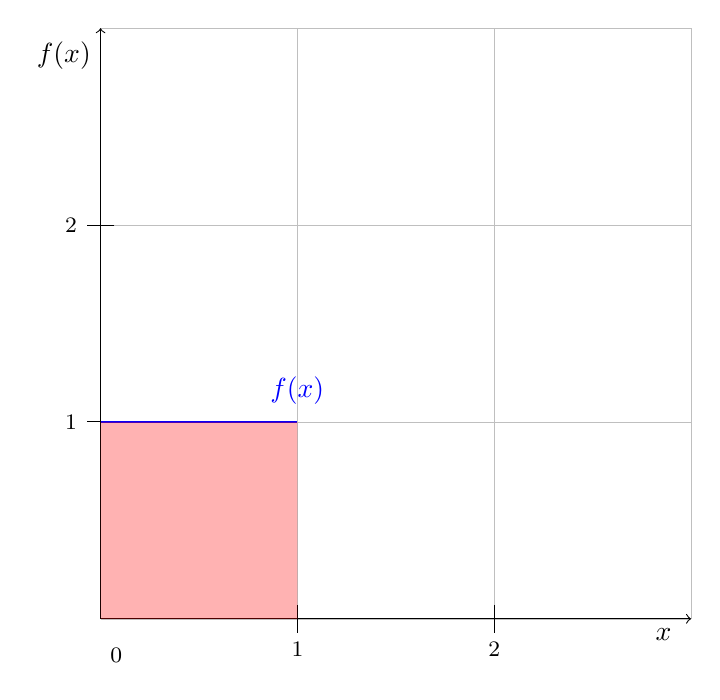
\begin{tikzpicture}[xscale=2.5, yscale=2.5]
	
	% Gitternetzlinien
	\draw[xstep=1cm, ystep=1cm, very thin, color=lightgray] (0,3) grid (3,0);
	% x-Achse
	\draw[->] (0,0) -- (3,0) node[below,xshift=-1em] {$x$}; 
	%Zahlen auf x-Achse
	%\foreach \x in {-2,...,-1}
	%\draw[shift={(\x,0)},color=black] (0pt,2pt) -- (0pt,-2pt) node[below] {\footnotesize $\x$};
	\foreach \x in {1,...,2}
	\draw[shift={(\x,0)},color=black] (0pt,2pt) -- (0pt,-2pt) node[below] {\footnotesize $\x$};
	% y-Achse 
	\draw[->] (0,0) -- (0,3) node[left,yshift=-1em] {$f(x)$};%node[above left]
	%Zahlen auf y-Achse
	%\foreach \y in {-1,...,-1}
	%\draw[shift={(0,\y)},color=black] (2pt,0pt) -- (-2pt,0pt) node[left] {\footnotesize $\y$};
	\foreach \y in {1,...,2}
	\draw[shift={(0,\y)},color=black] (2pt,0pt) -- (-2pt,0pt) node[left] {\footnotesize $\y$};
	%Ursprung
	\draw[color=black] (0pt,-5.3pt) node[right] {\footnotesize $0$};
	
	\draw[thick,color=blue] plot[samples=200, domain=0:1] 
	(\x,{1 }) node[below, yshift=2em] {$f(x)$};
	
	\fill[color =red,fill opacity=0.3] plot[domain=0:1] (\x,{(1 })% 
	-- plot[domain=1:0] (\x,{0});% 
	
	
	
	\end{tikzpicture}\\
\end{center}
\begin{align*}
\int\limits_{0}^{1} f(x)=1\cdot 1=1
\end{align*}
\newpage
\noindent
(ii) $ f:[0,2] \longmapsto \mathbb{R} $ mit $ x\longmapsto x $\\
\begin{center}
	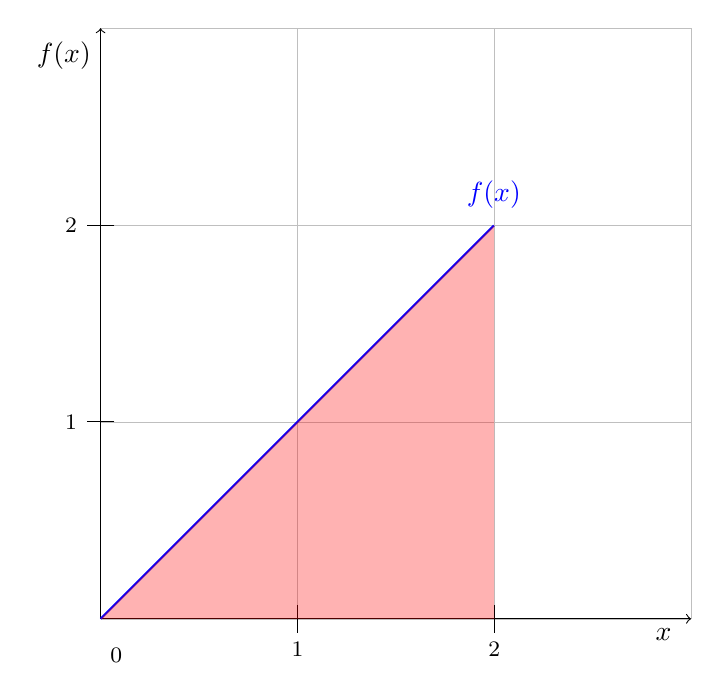
\begin{tikzpicture}[xscale=2.5, yscale=2.5]
	
	% Gitternetzlinien
	\draw[xstep=1cm, ystep=1cm, very thin, color=lightgray] (0,3) grid (3,0);
	% x-Achse
	\draw[->] (0,0) -- (3,0) node[below,xshift=-1em] {$x$}; 
	%Zahlen auf x-Achse
	%\foreach \x in {-2,...,-1}
	%\draw[shift={(\x,0)},color=black] (0pt,2pt) -- (0pt,-2pt) node[below] {\footnotesize $\x$};
	\foreach \x in {1,...,2}
	\draw[shift={(\x,0)},color=black] (0pt,2pt) -- (0pt,-2pt) node[below] {\footnotesize $\x$};
	% y-Achse 
	\draw[->] (0,0) -- (0,3) node[left,yshift=-1em] {$f(x)$};%node[above left]
	%Zahlen auf y-Achse
	%\foreach \y in {-1,...,-1}
	%\draw[shift={(0,\y)},color=black] (2pt,0pt) -- (-2pt,0pt) node[left] {\footnotesize $\y$};
	\foreach \y in {1,...,2}
	\draw[shift={(0,\y)},color=black] (2pt,0pt) -- (-2pt,0pt) node[left] {\footnotesize $\y$};
	%Ursprung
	\draw[color=black] (0pt,-5.3pt) node[right] {\footnotesize $0$};
	
	\draw[thick,color=blue] plot[samples=200, domain=0:2] 
	(\x,{\x }) node[below, yshift=2em] {$f(x)$};
	
	\fill[color =red,fill opacity=0.3] plot[domain=0:2] (\x,{(\x })% 
	-- plot[domain=2:0] (\x,{0});% 
	
	
	
	\end{tikzpicture}\\	
\end{center}
\begin{align*}
\int\limits_{0}^{2}f(x) \mathrm{d}x=\int\limits_{0}^{2} x\cdot \mathrm{d}x=\frac{1}{2}2^2=2
\end{align*}
\subsection{Das unbestimmte Integral}
\href{https://youtu.be/D5fcNNAZP2A}{Video 02}\\
Sei $ f:[a,b]\longmapsto \mathbb{R} $ integrierbar. Weiter sei $ x\in[a,b] $.\\
Wir definieren als unbestimmtes Integral von $ f $ auf $ [a,b] $:\\
\begin{align*}
\mathrm{F}(x):=\int\limits_{a}^{x} f(t)\mathrm{d}t
\end{align*}
Wir erhalten eine Abbildung:\\
\begin{align*}
\mathrm{F}:[a,b]\longmapsto \mathbb{R}\;\;\text{mit }\;\;x\longmapsto \int\limits_{a}^{x} f(t)\mathrm{d}t
\end{align*}
Beispiel:\\
Wir betrachten:\\
\begin{align*}
f:[0,10]\longmapsto \mathbb{R}\;\;\text{mit }\;\; f(t)=t\\
\end{align*}
Dann ist:\\
\begin{align*}
\mathrm{F}:[0,10]\longmapsto \mathbb{R}\;\;\text{mit }\;\; \mathrm{F}(x)=\int\limits_{0}^{x}f(t)\mathrm{d}t=\int\limits_{0}^{x} t\cdot \mathrm{d}t=\frac{x^2}{2}
\end{align*}
\begin{center}
	
	
	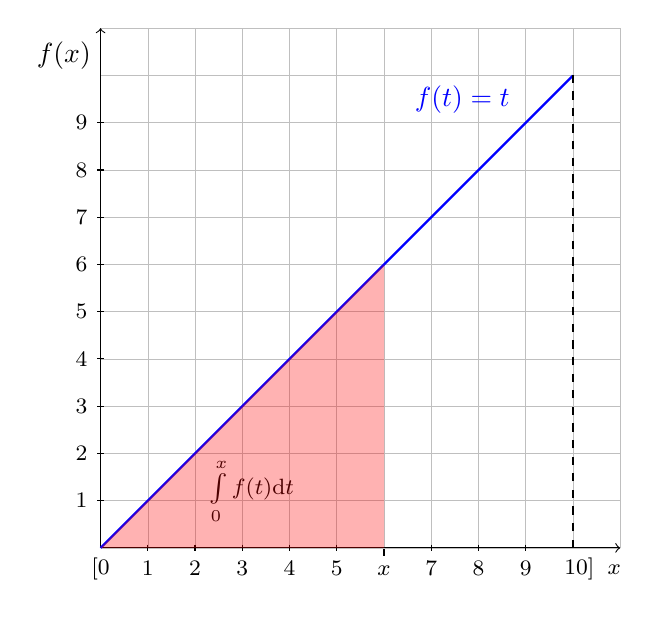
\begin{tikzpicture}[xscale=0.6, yscale=0.6]
	
	% Gitternetzlinien
	\draw[xstep=1cm, ystep=1cm, very thin, color=lightgray] (0,11) grid (11,0);
	% x-Achse
	\draw[->] (0,0) -- (11,0) node[below,xshift=-1em] {\footnotesize$10]\;\; x$}; 
		\draw (0,0)  node[below,xshift=0 em] {\footnotesize$[ 0$}; 
	%Zahlen auf x-Achse
	%\foreach \x in {-3,...,-1}
	%\draw[shift={(\x,0)},color=black] (0pt,2pt) -- (0pt,-2pt) node[below] {\footnotesize $\x$};
	\foreach \x in {1,...,5}
	\draw[shift={(\x,0)},color=black] (0pt,2pt) -- (0pt,-2pt) node[below] {\footnotesize $\x$};
	\foreach \x in {7,...,9}
	\draw[shift={(\x,0)},color=black] (0pt,2pt) -- (0pt,-2pt) node[below] {\footnotesize $\x$};
	% y-Achse 
	\draw[->] (0,0) -- (0,11) node[left,yshift=-1em] {$f(x)$};%node[above left]
	%Zahlen auf y-Achse
	%\foreach \y in {-1,...,-1}
	%\draw[shift={(0,\y)},color=black] (2pt,0pt) -- (-2pt,0pt) node[left] {\footnotesize $\y$};
	\foreach \y in {1,...,9}
	\draw[shift={(0,\y)},color=black] (2pt,0pt) -- (-2pt,0pt) node[left] {\footnotesize $\y$};
	%Ursprung
	%\draw[color=black] (0pt,-10pt) node[right] {\footnotesize $0$};
	
	\draw[shift={(6,-0.1)},color=black] (0pt,2pt) -- (0pt,-2pt) node[below] {\footnotesize $x$};
	
	\draw[color=black] (3.2,1.2) node {\footnotesize $\int\limits_{0}^{x} f(t)\mathrm{d}t$};
	
	\draw[thick,color=blue] plot[samples=200, domain=0:10] 
	(\x,{\x }) node[below, xshift=-4em] {$f(t)=t$};
	\fill[color =red,fill opacity=0.3] plot[domain=0:6] (\x,{(\x })% 
	-- plot[domain=6:0] (\x,{0});% 
\draw[color=black,thick,dashed] (10,0)--(10,10);
	\end{tikzpicture}\\
	\begin{align*}
	\int\limits_{0}^{x} f(t)\mathrm{d}t=\frac{1}{2}x^2
	\end{align*}
\end{center}
Bemerkung:\\
\begin{align*}
\mathrm{F}'(x)=\bigg(\frac{x^2}{2}\bigg)'=\frac{2x}{2}=x=f(x)\\
\end{align*}
\subsection{Der Hauptsatz der Differential- und Integralrechnung}
\href{https://youtu.be/2v6KdCjGNc0}{Video 03}\\
Sei $ f: \mathbb{I}\longmapsto \mathbb{R} $ stetig auf dem Intervall $  \mathbb{I} $ und $ a\in \mathbb{I} $, dann gilt:\\
(i) Ist F eine Stammfunktion von $ f $, dann gilt:\\
\begin{align*}
\mathrm{F}'(x)=\bigg(\int\limits_{a}^{x}f(t)\mathrm{d}t \bigg)'=f(x)
\end{align*}
(ii)\;Sei $ \mathrm{G}:[a,b]\longmapsto \mathbb{R} $ diffbar mit $ \mathrm{G}'=f(x) $, dann gilt:\\
\begin{align*}
\mathrm{G}=\int\limits_{a}^{x} f(t)\mathrm{d}t+\alpha\;\;\text{mit }\;\;\alpha\in\mathbb{R}
\end{align*}
(iii)\; Sei G eine Stammfunktion von $ f $ und $  \mathbb{I}=[a,b] $, dann ist das Integral:\\
\begin{align*}
\int\limits_{a}^{b} f(x)\mathrm{d}x=\mathrm{G}(b)-G(a)=\bigg[\mathrm{G}(x)\bigg]^b_a
\end{align*}
\newpage
Betracht: $ f:[0,2]\longmapsto\mathbb{R} $ mit $ f(x)=x^2 $ \\
\begin{quote}
	$\blacktriangleright$ Stammfunktion von $ f $\\
	\begin{quote}
		\begin{align*}
		\mathrm{F}'_1=\bigg(\frac{x^3}{3}\bigg)'=\frac{3}{3}\cdot x^2=f(x)
		\end{align*}
		D.h. $ \mathrm{F}_1 $ ist Stammfunktion von $ f $.
		\begin{align*}
		\mathrm{F}'_2=\bigg(\frac{x^3}{3}+12\bigg)'=\frac{3}{3}\cdot x^2=f(x)
		\end{align*}
		$ \mathrm{F}_2 $ ist ebenfals Stammfunktion von $ f $.
	\end{quote}
	$\blacktriangleright\;\;\mathrm{G}_\alpha(x)=\frac{x^3}{3}+\alpha$ 
	\begin{align*}
	\int\limits_{0}^{2} f(x)\mathrm{d}x=\mathrm{F}_2(2)-\mathrm{F}_2(0)=\frac{2^3}{3}+12-\bigg(\frac{0^3}{3}+12\bigg)=\frac{2^3}{3}=\frac{8}{3}
	\end{align*}
	Die Konstante $ \alpha $ hebt sich durch die Differenz auf.\\
	D.h.: Bei der Stammfunktion ist $ \alpha $ bei der Flächenberechnung nicht notwendig.\\
	\begin{align*}
	\int\limits_{0}^{2} f(x)\mathrm{d}x=\int\limits_{0}^{2} x^2\mathrm{d}x=\bigg[\frac{x^3}{3}\bigg]^2_0=\frac{2^3}{3}-\frac{0^3}{3}=\frac{8}{3}
	\end{align*}
\end{quote}
Bemerkung:\\
Aus dem Hauptsatz folgt: Integrieren und Differenzieren sind Gegenoperationen.\\
\subsubsection{Aufgabe 1 zum Hauptsatz der Differential- und Integralrechnung}
\href{https://youtu.be/yEC_tlNWT7E}{Video 04}\\
Berechne das folgende Integral:\\
\begin{align*}
\int\limits_{-1}^{1} (x^2+2x-7x)\mathrm{d}x
\end{align*}
Gesucht: $ \mathrm{F}(x) $ mit $ \mathrm{F}'(x)=f(x)=x^2+2x-7 $\\
\\
NR.:\\
Es gilt für die Ableitung von $ x^n \;\;\text{mit }\;\;n\in\mathbb{N} $:\\
\begin{align*}
\big(x^n\big)'=n\cdot x^{n-1}
\end{align*}
\newpage
Es gilt dann in die andere Richtung: Die Ableitung von F muss $ f(x) $ ergeben.\\
\begin{center}
	
	
	\renewcommand{\arraystretch}{1.4}
	\( \begin{array}{l|c} f(x)&\mathrm{F}\\
	\hline x^2&\frac{x^3}{3}\\
	x^3&\frac{x^4}{4}\\
	x^n&\frac{x^{n+1}}{n+1}
	\end{array} \)
	\begin{align*}
	\Rightarrow \mathrm{F}(x)=\frac{x^{n+1}}{n+1}
	\end{align*}
\end{center}
\begin{align*}
\mathrm{F}(x)= \mathrm{F}'(x)=f(x)&=x^2+2x-7\\
\mathrm{F}(x)&=\frac{x^{2+1}}{2+1}+2\cdot\frac{x^{1+1}}{1+1}-7\cdot\frac{x^{0+1}}{0+1}+\alpha\;\;\text{mit }\;\; \alpha\in\mathbb{R}\\
&=\frac{x^3}{3}+x^2-7x+\alpha\\
&=\bigg[\frac{x^3}{3}+x^2-7x\bigg]^1_{-1}=\frac{1}{3}+1-7-\bigg(-\frac{1}{3}+1+7\bigg)=-\frac{17}{3}-\frac{23}{3}=-\frac{40}{3}\\
\end{align*}
\subsubsection{ Aufgabe 2 zum Hauptsatz der Differential- und Integralrechnung}
\href{https://youtu.be/O-x6XCl7v-c}{Video 05}\\
Berechne folgende Integrale:\\
(i)\;\;$ \int\limits_{0}^{\pi} (\cos(x)+1) $\\
(ii)\;$ \int\limits_{1}^{2} \big(\sqrt{x}+\frac{4}{x}\big)$ \\
\\
zu (i):\\
\begin{align*}
&\int\limits_{0}^{\pi} (\cos(x)+1)\\
&\mathrm{F}(x)=\bigg[\sin(x)+x\bigg]^\pi_0=(\sin(\pi)+\pi)-(\sin(0)+0)=\pi\\
\end{align*}
zu (ii):\\
\begin{quote}
	
	\begin{align*}
	\int\limits_{1}^{2} \bigg(\sqrt{x}+\frac{4}{x}\bigg)
	\end{align*}
	NR.:\\
	\begin{align*}
	\sqrt{x}=x^{\frac{1}{2}}\\
	\end{align*}
	Exponent um 1 erhöhen:\\
	\begin{align*}
	x^{\frac{3}{2}}
	\end{align*}
	Davon die Ableitung:\\
	\begin{align*}
	\bigg(x^{\frac{3}{2}}\bigg)'=\frac{3}{2}\cdot x^{\frac{1}{2}}\\
	\end{align*}
	Die Ableitung soll aber $ x^{\frac{1}{2}} $ sein, deswegen $ x^{\frac{2}{3}} $mit $ \frac{2}{3} $ multiplitieren und dies ergibt dann:\\
	\begin{align*}
	\bigg(\frac{2}{3}x^{\frac{3}{2}}\bigg)'=x^{\frac{1}{2}}
	\end{align*}
\end{quote}
\begin{align*}
\mathrm{F}(x)&=\bigg[\frac{2}{3}x^{\frac{3}{2}}+4\ln(x)\bigg]^2_1\\
&=\frac{2}{3}\sqrt[2]{2^3}+4\ln(2)-\frac{2}{3}+0\\
&=\frac{2}{3}\sqrt{8}+4\ln(2)-\frac{2}{3}
\end{align*}
\subsubsection{ Aufgabe 1 zur Berechnung der Stammfunktion}
\href{https://youtu.be/bMi4SyWZKcg}{Video 06}\\
Bestimme die Stammfunktionen von:\\
\begin{align*}
f(x)=\frac{x^2-2x-3}{x-3}
\end{align*}
D.h.: Berechne alle $\mathrm{F}_\alpha$ mit $ \mathrm{F}'=f(x) $\\
Vom Zähler die Nullstellenberechnen (einfach probieren oder pq-Formel):\\
\begin{align*}
x^2-2x-3&=0\\
x_1&=3\\
x_2&=-1
\end{align*}
Die 3 ist eine Nullstelle und $ (x-3) $ teilt den Zähler.\\
Die -1 ist die zweite Nullstelle. Daraus folgt dann:\\
\begin{align*}
f(x)=\frac{x^2-2x-3}{x-3}=\frac{(x-3)(x+1)}{x-3}=x+1
\end{align*}
Die Stammfunktionen sind dann von $ f(x)=x+1 $:\\
\begin{align*}
\mathrm{F}_\alpha(x)=\frac{x^2}{2}+x+\alpha\;\;\text{mit }\;\; \alpha\in\mathbb{R}
\end{align*}
Prüfe:\
\begin{align*}
\mathrm{F}_\alpha'(x)=\bigg(\frac{x^2}{2}+x+\alpha\bigg)'=\frac{2}{2}x+1=x+1=f(x)
\end{align*}
\subsubsection{ Aufgabe 2 zur Berechnung der Stammfunktion}
\href{https://youtu.be/hunCkb-iq2Q}{Video 07}\\
Bestimme alle Stammfunktionen von:\\
\begin{align*}
g(x) =\sin(x)+\cos(x)
\end{align*}
Wir wissen:\\
\begin{align*}
\cos'(x)&=-\sin(x)\\
\sin'(x)&=\cos(x)
\end{align*}
Die Stammfunktionen sind dann von $ g(x)=\cos(x)+\sin(x) $:\\
\begin{align*}
\mathrm{G}_\alpha=-\cos(x)+\sin(x)+\alpha\;\;\text{mit }\;\; \alpha\in\mathbb{R}
\end{align*}
Prüfe:\\
\begin{align*}
\mathrm{G}'_\alpha=\bigg(-\cos(x)+\sin(x)+\alpha\bigg)'=\sin(x)+\cos(x)=g(x)
\end{align*}
\subsubsection{ Aufgabe 3 zur Berechnung der Stammfunktion}
\href{https://youtu.be/JBw8qcuJTRA}{Video 08}\\
Bestimme alle Stammfunktionen von:\\ 
\begin{align*}
h(x)=\frac{4}{x^3}+x^7\sqrt{x}
\end{align*}
Funktion $ h(x) $ in Potenzen umformen:\\
\begin{align*}
h(x)=4\cdot x^{-3}+x^7\cdot x^{\frac{1}{2}}=4x^{-3}+x^{\frac{15}{2}}
\end{align*}
Gesucht alle $ \mathrm{H}(x) $ mit $ \mathrm{H}'=h(x) $\\
Es gilt mit $ \mathrm{H}(x)=\frac{x^{n+1}}{n+1} $ oder durch Überlegung:\\
\begin{align*}
\mathrm{H}(x)&=4\cdot \frac{x^{(-3+1)}}{-3+1}+\frac{x^{(\frac{15}{2}+1)}}{\frac{15}{2}+1}\\
&=-2x^{-2}+\genfrac{}{}{}{2}{2 }{17}x^{\frac{17}{2}}
\end{align*}
\subsection{Rechenregeln/Eigenschaften   }
\subsubsection{Rechenregeln/Eigenschaften für das Integral I }
\href{https://youtu.be/aP327zIKmvI}{Video 09}\\
Seien $ f,g:[a,b] \longmapsto \mathbb{R}$ integrierbar, dann gilt für alle $ \lambda,\alpha\in\mathbb{R} $:\\
\begin{align*}
\int\limits_{a}^{b}\bigg( \lambda\cdot f(x)+\beta\cdot g(x)\bigg)=\lambda\int\limits_{a}^{b} f(x)\mathrm{d}x+\beta\int\limits_{a}^{b} g(x)\mathrm{d}x
\end{align*}
Beispiel:\\
\begin{align*}
\int\limits_{-1}^{1}(3x^2+7x) \mathrm{d}x&=3\cdot \int\limits_{-1}^{1} x^2\mathrm{d}x+7\cdot\int\limits_{-1}^{1} x\mathrm{d}x\\
&=3\bigg[\frac{x^3}{3}\bigg]^1_{-1}+7\bigg[\frac{x^2}{2}\bigg]^1_{-1}\\
&=3\bigg(\frac{1}{3}-\frac{-1}{3}\bigg)+7\bigg(\frac{1}{2}-\frac{1}{2}\bigg)\\
&=2
\end{align*}
oder:\\
\begin{align*}
\int\limits_{-1}^{1}(3x^2+7x) \mathrm{d}x&=\bigg[x^3+\frac{7}{2}x^2\bigg]^1_{-1}=2
\end{align*}
\newpage
\noindent
\subsubsection{Rechenregeln/Eigenschaften für das Integral II }
\href{https://youtu.be/bCqPDYJzXw0}{Video 10}\\
Seien $ f,g:[a,b]\longmapsto \mathbb{R} $.\\
Sei $ f(x)\leq g(x) $ für alle $ x\in [a,b] $, dann gilt:\\
\begin{align*}
\int\limits_{a}^{b}f(x)\mathrm{d}x\leq\int\limits_{a}^{b} g(x)\mathrm{d}x 
\end{align*}
Beispiel:\\
Es gilt:\\
\begin{align*}
f(x)=x^2\leq x = g(x)\;\;\text{mit }\;\;x\in[0,1]
\end{align*}
Für das Integral gilt dann:\\
\begin{align*}
\int\limits_{0}^{1} f(x)\mathrm{d}x&=\int\limits_{0}^{1} x^2\mathrm{d}x=\bigg[\frac{x^3}{3}\bigg]^1_0=\frac{1}{3}\\
\int\limits_{0}^{1}g(x)\mathrm{d}x&=\int\limits_{0}^{1} x\mathrm{d}x=\bigg[\frac{x^2}{2}\bigg]^1_0=\frac{1}{2}\\
\Rightarrow&\frac{1}{2}>\frac{1}{3}
\end{align*}
\newpage
\subsubsection{Rechenregeln/Eigenschaften für das Integral III }
\href{https://youtu.be/3EPUbiOtG2g}{Video 11}\\
Seien $ f,g:[a,b]\longmapsto \mathbb{R} $.\\
Es gilt:\\
\begin{align*}
\bigg|\int\limits_{a}^{b} f(x)\mathrm{d}x\bigg|\leq \int\limits_{a}^{b}\big|f(x)\big| 
\end{align*}
Beispiel: $ f(x)=\sin(x) $\\

$\bullet$ Für das Integral: $ \bigg|\int\limits_{0}^{2\pi} \sin(x)\mathrm{d}x\bigg| $ gilt:\\

\begin{align*}
\bigg|\int\limits_{0}^{2\pi} \sin(x)\mathrm{d}x\bigg|=\bigg|\bigg[-\cos(x)\bigg]^{2\pi}_0\bigg|=(-\cos(2\pi)-\big(-cos(0)\big)=\big|-1+1\big|=0\\
\end{align*}
\begin{center}
	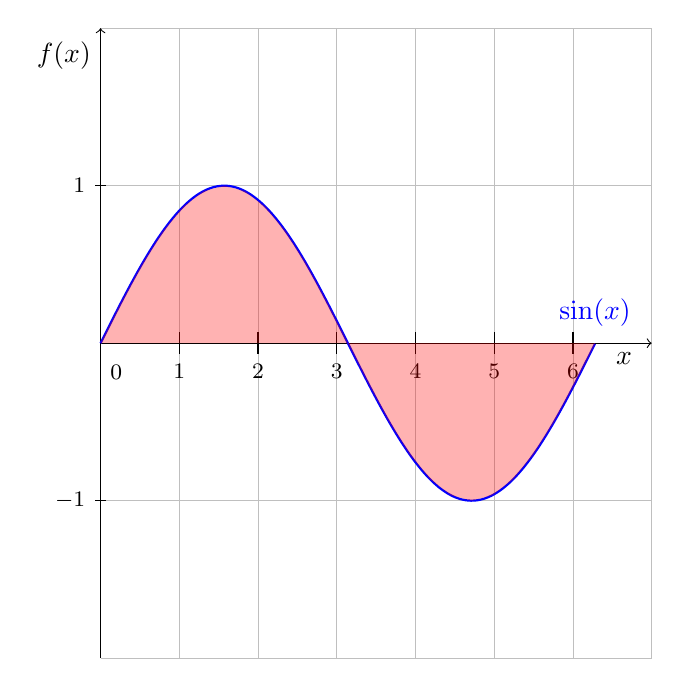
\begin{tikzpicture}[xscale=1, yscale=2]
	
	% Gitternetzlinien
	\draw[xstep=1cm, ystep=1cm, very thin, color=lightgray] (0,2) grid (7,-2);
	% x-Achse
	\draw[->] (0,0) -- (7,0) node[below,xshift=-1em] {$x$}; 
	%Zahlen auf x-Achse
	%\foreach \x in {-2,...,-6}
	%\draw[shift={(\x,0)},color=black] (0pt,2pt) -- (0pt,-2pt) node[below] {\footnotesize $\x$};
	\foreach \x in {1,...,6}
	\draw[shift={(\x,0)},color=black] (0pt,2pt) -- (0pt,-2pt) node[below] {\footnotesize $\x$};
	% y-Achse 
	\draw[->] (0,-2) -- (0,2) node[left,yshift=-1em] {$f(x)$};%node[above left]
	%Zahlen auf y-Achse
	\foreach \y in {-1,...,-1}
	\draw[shift={(0,\y)},color=black] (2pt,0pt) -- (-2pt,0pt) node[left] {\footnotesize $\y$};
	\foreach \y in {1,...,1}
	\draw[shift={(0,\y)},color=black] (2pt,0pt) -- (-2pt,0pt) node[left] {\footnotesize $\y$};
	%Ursprung
	\draw[color=black] (0pt,-5.3pt) node[right] {\footnotesize $0$};
	
	\draw[thick,color=blue] plot[samples=200, domain=0:6.28] 
	(\x,{(sin(\x r)  }) node[below, yshift=2em] {$\sin(x)$};
	
	\fill[color =red,fill opacity=0.3] plot[domain=0:6.28] (\x,{(sin(\x r) })% 
	-- plot[domain=6.28:0] (\x,{0});% 
	
	
	
	\end{tikzpicture}\\	
\end{center}

$\bullet$ Für das Integral: $ \int\limits_{0}^{2\pi}\big| \sin(x)\mathrm{d}x\big| $ gilt:\\
\begin{align*}
\int\limits_{0}^{2\pi}\big| \sin(x)\mathrm{d}x\big| =2\int\limits_{0}^{\pi} \sin(x)\mathrm{d}x=\bigg[-\cos(x)\bigg]^{\pi}_0=2\big(-\cos(\pi)-(-\cos(0)\big)=2\cdot 2=4
\end{align*}
\begin{center}
	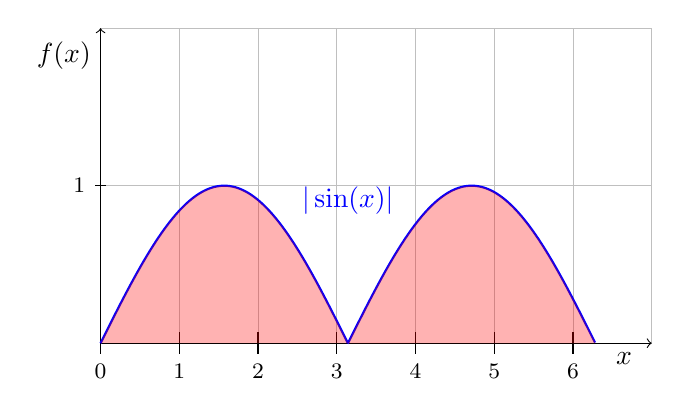
\begin{tikzpicture}[xscale=1, yscale=2]
	
	% Gitternetzlinien
	\draw[xstep=1cm, ystep=1cm, very thin, color=lightgray] (0,2) grid (7,0);
	% x-Achse
	\draw[->] (0,0) -- (7,0) node[below,xshift=-1em] {$x$}; 
	%Zahlen auf x-Achse
	%\foreach \x in {-2,...,-6}
	%\draw[shift={(\x,0)},color=black] (0pt,2pt) -- (0pt,-2pt) node[below] {\footnotesize $\x$};
	\foreach \x in {0,...,6}
	\draw[shift={(\x,0)},color=black] (0pt,2pt) -- (0pt,-2pt) node[below] {\footnotesize $\x$};
	% y-Achse 
	\draw[->] (0,0) -- (0,2) node[left,yshift=-1em] {$f(x)$};%node[above left]
	%Zahlen auf y-Achse
	%\foreach \y in {-1,...,-1}
	%\draw[shift={(0,\y)},color=black] (2pt,0pt) -- (-2pt,0pt) node[left] {\footnotesize $\y$};
	\foreach \y in {1,...,1}
	\draw[shift={(0,\y)},color=black] (2pt,0pt) -- (-2pt,0pt) node[left] {\footnotesize $\y$};
	%Ursprung
	%\draw[color=black] (0pt,-5.3pt) node {\footnotesize $0$};
	
	\draw[thick,color=blue] plot[samples=200, domain=0:3.14] 
	(\x,{(sin(\x r)  }) node[below, yshift=6em] {$|\sin(x)|$};
	\draw[thick,color=blue] plot[samples=200, domain=3.14:6.28] 
	(\x,{(cos((\x+1.57) r)  });
	\fill[color =red,fill opacity=0.3] plot[domain=0:3.14] (\x,{(sin(\x r) })% 
	-- plot[domain=6.28:0] (\x,{0});% 
	
	\fill[color =red,fill opacity=0.3] plot[domain=3.14:6.28] (\x,{(cos((\x+1.57) r) })% 
	-- plot[domain=6.28:3.14] (\x,{0});% 
	
	\end{tikzpicture}\\	
\end{center}
\subsubsection{Rechenregeln/Eigenschaften für das Integral IV u. V }
\href{https://youtu.be/O5sAZWsINYo}{Video 12}\\
Seien $ f,g:[a,b]\longmapsto \mathbb{R} $.\\
Es gilt:\\
$ \bullet \int\limits_{a}^{b} f(x)=\int\limits_{a}^{\alpha}f(x)+\int\limits_{\alpha}^{b}f(x)\mathrm{d}x \;\;\;\; $ mit\;\; $ \alpha\in[a,b] $\\
\begin{center}
	
	
	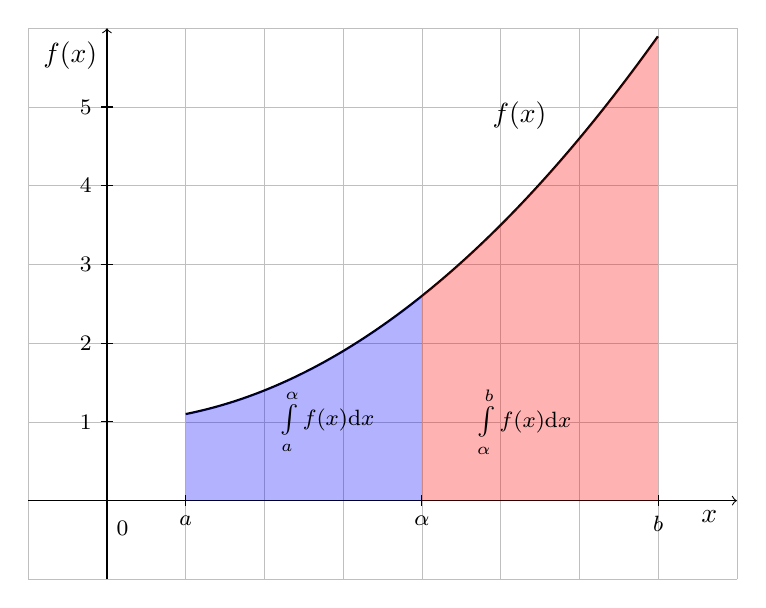
\begin{tikzpicture}[xscale=1, yscale=1]
	
	% Gitternetzlinien
	\draw[xstep=1cm, ystep=1cm, very thin, color=lightgray] (-1,6) grid (8,-1);
	% x-Achse
	\draw[->] (-1,0) -- (8,0) node[below,xshift=-1em] {$x$}; 
	%Zahlen auf x-Achse
	%\foreach \x in {-3,...,-1}
	%\draw[shift={(\x,0)},color=black] (0pt,2pt) -- (0pt,-2pt) node[below] {\footnotesize $\x$};
	%\foreach \x in {a,...,7}
	%\draw[shift={(\x,0)},color=black] (0pt,2pt) -- (0pt,-2pt) node[below] {\footnotesize $\x$};
	
	% y-Achse 
	\draw[->] (0,-1) -- (0,6) node[left,yshift=-1em] {$f(x)$};%node[above left]
	%Zahlen auf y-Achse
	%\foreach \y in {-1,...,-1}
	%\draw[shift={(0,\y)},color=black] (2pt,0pt) -- (-2pt,0pt) node[left] {\footnotesize $\y$};
	\foreach \y in {1,...,5}
	\draw[shift={(0,\y)},color=black] (2pt,0pt) -- (-2pt,0pt) node[left] {\footnotesize $\y$};
	%Ursprung
	\draw[color=black] (0pt,-10pt) node[right] {\footnotesize $0$};
	
	\draw[thick,color=black] plot[samples=200, domain=1:7] 
	(\x,{0.1*\x^2+1}) node[below, xshift=-5em,yshift=-2em] {$f(x)$};
	
	\fill[color =blue,fill opacity=0.3] plot[domain=1:4] (\x,{(0.1*\x^2+1 })% 
	-- plot[domain=4:1] (\x,{0});% 
	\fill[color =red,fill opacity=0.3] plot[domain=4:7] (\x,{(0.1*\x^2+1 })% 
	-- plot[domain=7:4] (\x,{0});% 
	\draw[shift={(1,0)},color=black] (0pt,2pt) -- (0pt,-2pt) node[below] {\footnotesize $a$};
	\draw[shift={(4,0)},color=black] (0pt,2pt) -- (0pt,-2pt) node[below] {\footnotesize $\alpha$};
	\draw[shift={(7,0)},color=black] (0pt,2pt) -- (0pt,-2pt) node[below] {\footnotesize $b$};
	\draw[color=black] (5.3,1) node {\footnotesize $\int\limits_{\alpha}^{b} f(x)\mathrm{d}x$};
	\draw[color=black] (2.8,1) node {\footnotesize $\int\limits_{a}^{\alpha} f(x)\mathrm{d}x$};
	\end{tikzpicture}\\
\end{center}
Beispiel:\\
\begin{align*}
\int\limits_{0}^{2}x\mathrm{d}x=\int\limits_{0}^{1} x\mathrm{d}x +\int\limits_{1}^{2}x\mathrm{d}x
\end{align*}
\newpage
\noindent
Es gilt:\\
$\bullet  \int\limits_{a}^{b}f(x) \mathrm{d}x=-\int\limits_{b}^{a}f(x)\mathrm{d}x  $ 
Beispiel:\\
\begin{align*}
\int\limits_{0}^{1} 1x=\big[x\big]^1_0=1\\
\int\limits_{1}^{0} 1x=\big[x\big]^0_1=-1\\
\end{align*}
\subsection{Integrationsregeln}
\subsubsection{Partielle Integration }
\href{https://youtu.be/bsTdvvGm7Ic}{Video 13}\\
Seien $ u,v:[a,b]\longmapsto \mathbb{R} $ diffbar und $ u', v' $ stetig, dann gilt:\\
\begin{align*}
\big(u(x)\cdot v(x)\big)'&=u'(x)\cdot v(x) +u(x)\cdot v'(x)\\
\Leftrightarrow \int\limits_{}^{}\big(u(x)\cdot v(x)\big)'\mathrm{d}x  &=\int\limits_{}^{}u'(x)\cdot v(x)+\int\limits_{}^{}u(x)\cdot v'(x)  \\
\end{align*}
$ \Leftrightarrow $ Achtung: Die Äquifallenz ist hier wegen den Konstanten nicht korrekt.\\
\begin{align*}
\int\limits_{}^{}\big(u(x)\cdot v(x)\big)'\mathrm{d}x  &=\int\limits_{}^{}u'(x)\cdot v(x)+\int\limits_{}^{}u(x)\cdot v'(x)  \\
u(x)\cdot v(x)  &=\int\limits_{}^{}u'(x)\cdot v(x)+\int\limits_{}^{}u(x)\cdot v'(x)  \\
\Leftrightarrow u(x)\cdot v(x)-\int\limits_{}^{}u'(x)\cdot v(x)&=\int\limits_{}^{}u(x)\cdot v'(x)  \\
\end{align*}
Für die partielle Integration gilt dann mit Integrationsgrenzen:\\
\begin{center}
	\fbox{\parbox  {80mm} {$\big[u(x)\cdot v(x)\big]^b_a-\int\limits_{a}^{b}u'(x)\cdot v(x)=\int\limits_{a}^{b}u(x)\cdot v'(x)   $}}
\end{center}
\subsubsection{Beispiel zur partiellen Integration }
\href{https://youtu.be/92SY1mE5hrMvv}{Video 14}\\
Berechne das Integral:\\
\begin{align*}
\int\limits_{0}^{1} x \mathrm{e}^x\mathrm{d}x
\end{align*}
Man wählt vorteilhaft $ u(x), v'(x) $:\\
\begin{align*}
u(x)=x&\Rightarrow u'(x)=1\\
v'(x)=\mathrm{e}^x&\Rightarrow v(x)=e^x
\end{align*}
Nun gilt:\\
\begin{align*}
\int\limits_{a}^{b}u(x)\cdot v'(x) =\big[u(x)\cdot v(x)\big]^b_a-\int\limits_{a}^{b}u'(x)\cdot v(x) 
\end{align*}
Dann einsetzen von $ u(x), u'(x), v(x), v'(x) $:\\
\begin{align*}
\int\limits_{0}^{1} x\mathrm{e}^x&=\bigg[x\cdot \mathrm{e}^x\bigg]^1_0-\int\limits_{a}^{b} 1\cdot\mathrm{e}^x \mathrm{d}x\\
&=\bigg[x\cdot \mathrm{e}^x\bigg]^1_0-\bigg[\mathrm{e}^x\bigg]_0^1\\
&=\mathrm{e}-0\mathrm{e}^0-(\mathrm{e}-1)\\
&=\mathrm{e}-\mathrm{e}+1=1
\end{align*}
Damit man sich die Formel nicht merken muß, kann man sich merken:\\
Bilde $ u(x) $ und $ v'(x) $ und notiere dies tabelarisch:\\
\begin{align*}
u(x)&\Rightarrow u'(x)\\
v'(x)&\Rightarrow v(x)
\end{align*}
Die Diagonale ergibt den Term: $\big[u(x)\cdot v(x)\big]^b_a  $\\
Die zweit Spalte ergibt den Term:$ \int\limits_{a}^{b}u'(x)\cdot v(x) $
\subsubsection{Trick I zur partiellen Integration }
\href{https://youtu.be/EM79gyqz1yo}{Video 15}\\
Bestimme alle Stammfunktionen von:\\
\begin{align*}
f(x)=x^2\cdot \mathrm{e} ^x
\end{align*}
Berechne:\\
\begin{align*}
\mathrm{F}(x)=\int\limits_{}^{} f(x)\mathrm{d}x=\int\limits_{}^{} x^2\cdot \mathrm{e}^x\mathrm{d}x
\end{align*}
NR.:\\
\begin{align*}
u(x)=x^2&\Rightarrow u'(x)=2x\\
v'(x)=\mathrm{e}^x&\Rightarrow v(x)=e^x\\
\end{align*}
\begin{align*}
\int\limits_{}^{}x^2\cdot \mathrm{e}^x\mathrm{d}x&= x^2\cdot \mathrm{e}^x-\int\limits_{}^{} 2x\mathrm{e}^x\mathrm{d}x\\
&=x^2\cdot \mathrm{e}^x-2\int\limits_{}^{} x\cdot \mathrm{e}^x\mathrm{d}x\\
\end{align*}
Berechnung vom Integral $\int\limits_{}^{}x\cdot \mathrm{e}^x\mathrm{d}x  $:\\
\begin{align*}
u(x)=x&\Rightarrow u'(x)=1\\
v'(x)=\mathrm{e}^x&\Rightarrow v(x)=\mathrm{e}^x
\end{align*}
\begin{align*}
\int\limits_{}^{} x\cdot \mathrm{e}^x=x \cdot \mathrm{e}^x-\int\limits_{}^{}\mathrm{e}^x\mathrm{d}x=x\cdot \mathrm{e}^x-\mathrm{e}^x 
\end{align*}
Dies ergibt dann eingesetzt:\\
\begin{align*}
\int\limits_{}^{} x^2\cdot \mathrm{e}^x\mathrm{d}x&=x^2\cdot \mathrm{e}^x-2(x\cdot \mathrm{e}^x-\mathrm{e}^x)\\
&=x^2\cdot \mathrm{e}^x-2\cdot(x-1)\\
&=x^2\cdot \mathrm{e}^2-2\cdot\mathrm{e}^x\cdot x+2\cdot \mathrm{e}^x\\
&=\mathrm{e}^x(x^2-2x+2)
\end{align*}
Es reicht wenn man jetzt erst mit den Konstanten rechnet um alle Stammfunktionen zu bekommen:\\
Fazit:\\
Alle Stammfunktionen von $ f(x) $ sind:\\
\begin{align*}
\mathrm{F}_\alpha=\mathrm{e}^x(x^2-2x+2) +\alpha\;\;\text{mit }\;\;\alpha\in\mathbb{R}
\end{align*}





\subsubsection{Trick II zur partiellen Integration}
\href{https://youtu.be/TbMWPRG4Ffw}{Video 16}\\
Bestimme alle Stammfunktionen von:\\
\begin{align*}
\int\limits_{}^{}\ln(x)\mathrm{d}x
\end{align*}
\underline{Trick:}\\
\begin{align*}
\int\limits_{}^{} \ln(x)\mathrm{d}x=\int\limits_{}^{} 1\cdot \ln(x)\mathrm{d}x
\end{align*}
NR.:\
\begin{align*}
u(x)=\ln(x)&\Rightarrow u'(x)=\frac{1}{x}\\
v(x)=1&\Rightarrow v'(x)=x
\end{align*}
Dies ergibt dann:\\
\begin{align*}
\int\limits_{}^{} \ln(x)&=u(x) \cdot v'(x)-\int\limits_{}^{} u'(x)\cdot v'(x)\mathrm{d}x\\
&=x\cdot \ln(x)-\int\limits_{}^{} \frac{1}{x}\cdot x\mathrm{d}x\\
&=x\cdot \ln(x)-\int\limits_{}^{}1\mathrm{d}x\\
&=x\cdot \ln(x)-x\\
&=x(\ln(x)-1)
\end{align*}
Probe:\\
\begin{align*}
\bigg(x(\ln(x)-1)\bigg)'=1\cdot (\ln(x)-1)+x\cdot \frac{1}{x}=\ln(x)-1+1=\ln(x)\\
\end{align*}
\subsubsection{Trick III zur partiellen Integration}
\href{https://youtu.be/sKeTwFd3Gfw}{Video 17}\\
Bestimme alle Stammfunktionen von:\\
\begin{align*}
h(x)=\cos(x)\cdot \sin(x)
\end{align*}
Berechne das Integral von:\\
\begin{align*}
\int\limits_{}^{} h(x)\mathrm{d}x=\int\limits_{}^{} \cos(x)\cdot \sin(x)\mathrm{d}x
\end{align*}
NR.:\\
\begin{align*}
u(x)=\cos(x)&\Rightarrow u'(x)=-sin(x)\\
v'(x)=\sin(x)&\Rightarrow v(x)=-\cos(x)\\
\end{align*}
Dies ergibt dann:\\
\begin{align*}
\int\limits_{}^{} h(x)\mathrm{d}x=\int\limits_{}^{}\cos(x)\cdot \sin(x)\mathrm{d}x=\cos(x)\cdot -\cos(x)-\int\limits_{}^{} \cos(x)\cdot\sin(x)\mathrm{d}x\\
\end{align*}
Jetzt ist man nicht viel weiter gekommen. Mit Addition von $\int\limits_{}^{} \cos(x)\cdot\sin(x)\mathrm{d}x  $ links und rechts der Gleichung ergibt dann:\\
\begin{align*}
\int\limits_{}^{}\cos(x)\cdot \sin(x)\mathrm{d}x+\int\limits_{}^{} \cos(x)\cdot\sin(x)\mathrm{d}x& =-\cos^2(x)-\int\limits_{}^{} \cos(x)\cdot\sin(x)\mathrm{d}x+\int\limits_{}^{} \cos(x)\cdot\sin(x)\mathrm{d}x\\
2\int\limits_{}^{} \cos(x)\cdot \sin(x)\mathrm{d}x&=-\cos^2(x)\\
\Leftrightarrow \int\limits_{}^{} \cos(x)\cdot \sin(x)\mathrm{d}x &=-\frac{1}{2} \cos^2(x)
\end{align*}
Fazit:\\
Alle Stammfunktionen sind in der Form:\\
\begin{align*}
\int\limits_{}^{} \cos(x)\cdot \sin(x)\mathrm{d}x &=-\frac{1}{2} \cos^2(x)+\alpha \;\;\text{mit }\;\;\alpha\in\mathbb{R}
\end{align*}
\subsection{Substitution}
\subsubsection{Substitutionsregel}
\href{https://youtu.be/Gfg8adsiy84}{Video 18}\\
Sei F eine Stammfunktion der stetigen Funktion $ f $ und $ x(t) $ eine diffbare Funktion sowie $ x'(t) $ stetig.\\
\begin{align*}
\mathrm{F}(x(t))
\end{align*}
Bemerkung:\\
Die Ableitung von$ f'(x) =\frac{d}{\mathrm{d}x}f(x)$\\
Dann ergibt sich, wenn man $ \mathrm{F}(x(t)) $ ableitet:\\
\begin{align*}
\frac{d}{\mathrm{d}t}\big(\mathrm{F}(x(t))\big)=\mathrm{F}'(x(t))\cdot x'(t)=f(x(t))\cdot x'(t)
\end{align*}
Integriert man nun beide Seiten:\\
\begin{align*}
\int\limits_{}^{} \frac{d}{\mathrm{d}t}(\mathrm{F}(x(t)))\mathrm{d}t=\int\limits_{}^{} f(x(t))\cdot x'(t)\mathrm{d}t
\end{align*}
Das Integrieren und Differenzieren neutralisieren sich.\\
\begin{align*}
\mathrm{F}(x(t))=\int\limits_{}^{} f(x(t))\cdot x'(t)\mathrm{d}t
\end{align*}
Mit Grenzen gilt dann:\\
\begin{align*}
\mathrm{F}(x(b))-\mathrm{F}(x(a))=\int\limits_{a}^{b} f(x(t))\cdot x'(t)\mathrm{d}t
\end{align*}
\subsubsection{Beispiel zur Substitution}
\href{https://youtu.be/JLzCF3VnqkU}{Video 19}\\
Berechne:\\
\begin{align*}
\int\limits_{0}^{\frac{\pi}{2}}  \sin(2x) \mathrm{d}x
\end{align*}
NR.: Substition mit:
\begin{align*}
t=2x
\end{align*}
Dann erhält man:\\
\begin{align*}
\int\limits_{}^{} \sin(t)\mathrm{d}x
\end{align*}
Nun muß noch $ \mathrm{d}x $ von $ \mathrm{d}t $ abhängig werden.\\
\begin{align*}
t=2x\Rightarrow 
\end{align*}
Durch Ableiten nach $ \frac{\mathrm{d}t}{\mathrm{d}x} $ erhält man $ \mathrm{d}x $:\\
\begin{align*}
\frac{\mathrm{d}t}{\mathrm{d}x}&=\frac{\mathrm{d}2x}{\mathrm{d}x}=2\\
\Leftrightarrow\frac{\mathrm{d}t}{2}&=\mathrm{d}x
\end{align*}
So bekommt man das lösbare Integral:\\
\begin{align*}
\int\limits_{}^{} \sin(t)\frac{\mathrm{d}t}{2}
\end{align*}
Die neuen Grenzen sind dann:\\
Obergrenze mit $ x=\frac{\pi}{2} $:\\
\begin{align*}
t&=2x\\
t=&2\cdot \frac{\pi}{2}=\pi
\end{align*}
Untergrenze mit $x= 0 $:\\
\begin{align*}
t&=2x\\
t=&2\cdot 0=0
\end{align*}
Die neue Stammfunktion ist dann:\\
\begin{align*}
\int\limits_{0}^{\pi}\sin(t) \frac{\mathrm{d}t}{2}=\frac{1}{2}\bigg[-\cos(t)\bigg]^\pi_0=\frac{1}{2}\big(-\cos(\pi)-(-\cos(0)\big)=\frac{1}{2}\big(+1-(-1)\big)=\frac{2}{2}=1\\
\end{align*}
Jetzt die Berechnung, so dass man die Substitutionsregel erkennt:\\
NR.: Substitution mit:\\
\begin{align*}
x(t)=\frac{t}{2}\Rightarrow& \frac{\mathrm{d}x}{\mathrm{d}t}=\frac{\mathrm{d}t}{2\mathrm{d}t}=\frac{1}{2}\\
\Leftrightarrow&\mathrm{d}x(t)=\frac{\mathrm{d}t}{2}
\end{align*}
Dann erhält man durch einsetzen in $\int\limits_{}^{} \sin(2\cdot x(t))\mathrm{d}x(t) \mathrm{d}t=\int\limits_{}^{} \sin(2\cdot x(t))x' (t) \mathrm{d}t $:\\
\begin{align*}
\int\limits_{}^{} \sin\bigg(2\cdot \frac{t}{2}\bigg)\cdot \frac{\mathrm{d}t}{2}=\int\limits_{}^{} \sin(t)\frac{\mathrm{d}t}{2}\\
\end{align*}
Untere Grenze:\\
\begin{align*}
x=0=\frac{t}{2}=0
\end{align*}
Obere Grenze:\\
\begin{align*}
x=\frac{\pi}{2}=\frac{t}{2}\Rightarrow t=\pi
\end{align*}
Bemerkung:\\
Zuerst wurde $ t=2x $ substituiert und dies ist die Umkehrfunktion von $ x(t)=\frac{t}{2} $.
\subsubsection{Trick 1 zur Substitutionsregel Aufgabe 1}
\href{https://youtu.be/IjIGyA63qtU}{Video 20}\\
Berechne:\\
\begin{align*}
\int\limits_{1}^{2} \frac{x}{(4x-1)^3}\mathrm{d}x
\end{align*}
(Lineare) Substitution:\\
\begin{align*}
t=4x-1
\end{align*}
Nach $ x $ ableiten:\\
\begin{align*}
\frac{\mathrm{d}t}{\mathrm{d}x}&=\frac{d(4x-1)}{\mathrm{d}x}=4\\
\Leftrightarrow \frac{\mathrm{d}t}{4}&=\mathrm{d}x
\end{align*}
Dann erhält man das Integral:\\
\begin{align*}
\int\limits_{}^{} \frac{x}{t^3}\cdot \frac{\mathrm{d}t}{4}
\end{align*}
Das $ x $ durch $ t $ ersetzen:\\
\begin{align*}
t&=4x-1\\
\Leftrightarrow x&=\frac{t+1}{4}
\end{align*}
Dann erhält man:\\
\begin{align*}
\int\limits_{}^{} \frac{\frac{t+1}{4}}{t^3}\cdot \frac{\mathrm{d}t}{4}=\frac{1}{16}\int\limits_{}^{} \frac{t+1}{t^3}\mathrm{d}t
\end{align*}
Die neuen Grenzen berechnen:\\
\begin{quote}
	Untere Grenze:\\
	\begin{align*}
	x=1\Rightarrow t=4x-1=4\cdot 1-1=3
	\end{align*}
	Obere Grenze:\\
	\begin{align*}
	x=2\Rightarrow t=4x-1=4\cdot 2-1=7
	\end{align*}
\end{quote}
Das Integral ist dann:\\
\begin{align*}
\frac{1}{16}\int\limits_{3}^{7} \frac{t+1}{t^3}\mathrm{d}t&=\frac{1}{16}\int\limits_{3}^{7} \bigg(\frac{t}{t^3}+\frac{1}{t^3}\bigg)=\frac{1}{16}\int\limits_{3}^{7} \bigg(\frac{1}{t^2}+\frac{1}{t^3}\bigg)\\
&=\frac{1}{16}\bigg[-\frac{1}{t}-\frac{1}{2t^2}\bigg]^7_3\\
&=\frac{1}{16}\bigg[-\frac{1}{7}-\frac{1}{2\cdot 49}-\bigg(-\frac{1}{3}-\frac{1}{2\cdot 9}\bigg)\bigg]\\
&\cdots
\end{align*}
\subsubsection{Trick 1 zur Substitutionsregel Aufgabe 2}
\href{https://youtu.be/tlmzM6q92Lc}{Video 21}\\
Berechne:\\
\begin{align*}
\int\limits_{0}^{1} \frac{1}{(x-2)^4}\mathrm{d}x 
\end{align*}
Substitution:\\
\begin{align*}
t=x-2
\end{align*}
Nach $ x $ ableiten:\\
\begin{align*}
\frac{\mathrm{d}t}{\mathrm{d}x}&=\frac{d(x-2)}{\mathrm{d}x}=1\\
\Leftrightarrow \mathrm{d}t&=\mathrm{d}x
\end{align*}
Dann erhält man:\\
\begin{align*}
\int\limits_{}^{} \frac{1}{t^4}\mathrm{d}t
\end{align*}
Die neuen Grenzen berechnen:\\
\begin{quote}
	Untere Grenze:\\
	\begin{align*}
	x=0\Rightarrow t=x-2= 0-2=-2
	\end{align*}
	Obere Grenze:\\
	\begin{align*}
	x=1\Rightarrow t=x-2= 1-2=-1
	\end{align*}
\end{quote}
Das Integral ist dann:\\
\begin{align*}
\int\limits_{-2}^{-1} \frac{1}{t^4}\mathrm{d}t&=\bigg[-\frac{1}{3}\cdot\frac{1}{t^3}\bigg]^{-1}_2\\
&=-\frac{1}{3}\cdot\frac{1}{(-1)^3}-\bigg(-\frac{1}{3}\cdot\frac{1}{(-2)^3}\bigg)=\frac{1}{3}-\frac{1}{24}=\frac{8-1}{24}=\frac{7}{24}
\end{align*}
\subsubsection{Trick 2 zur Substitutionsregel}
\href{https://youtu.be/ECFaj8YJlws}{Video 22}\\
Berechne:\\
\begin{align*}
\int\limits_{0}^{\frac{\pi}{2}}\frac{\cos^3(x)}{1-\sin(x)} \mathrm{d}x
\end{align*}
Substitution:\\
\begin{align*}
t=&\sin(x)\\
\frac{\mathrm{d}t}{\mathrm{d}x}&=\frac{\mathrm{d}(\sin(x))}{\mathrm{d}x}=\cos(x)\\
\Leftrightarrow&\frac{\mathrm{d}t}{\cos(x)}=\mathrm{d}x\\
\end{align*}
Dann erhält man:\\
\begin{align*}
\int\limits_{}^{} \frac{\cos^3(x)}{1-t}\cdot\frac{\mathrm{d}t}{\cos(x)}=\int\limits_{}^{} \frac{\cos^2(x)}{1-t}\mathrm{d}t
\end{align*}
Es gilt:\\
\begin{align*}
&\cos^2(x)+\sin^2(x)=1\\
&\Leftrightarrow \cos^2(x)=1-\sin^2(x)
\end{align*}
Mit $ t=\sin(x) $ gilt dann:\\
\begin{align*}
\cos^2(x)=1-t^2
\end{align*}
Dann erhält man:\\
\begin{align*}
\int\limits_{}^{} \frac{1-t^2}{1-t}\mathrm{d}t
\end{align*}
Die neuen Grenzen berechnen:\\
\begin{quote}
	Untere Grenze:\\
	\begin{align*}
	x=0\Rightarrow t=\sin(0)=0
	\end{align*}
	Obere Grenze:\\
	\begin{align*}
	x=\frac{\pi}{2}\Rightarrow t=\sin\bigg(\frac{\pi}{2}\bigg)=1
	\end{align*}
\end{quote}
Das Integral ist dann:\\
\begin{align*}
\int\limits_{0}^{1} \frac{1-t^2}{1-t}\mathrm{d}t&=\int\limits_{0}^{1} \frac{(1-t)(1+t)}{1-t}\mathrm{d}t=\int\limits_{0}^{1}(1+t)\mathrm{d}t\\ 
&=\bigg[t+\frac{t^2}{2}\bigg]^1_0=\bigg(1+\frac{1}{2}\bigg)=\frac{3}{2}
\end{align*}
\subsubsection{Trick 3 zur Substitutionsregel}
\href{https://youtu.be/wque3ru-qwM}{Video 23}\\
Berechne:\\
\begin{align*}
\int\limits_{0}^{2} \frac{\sqrt{x^2+16}}{2}\cdot \mathrm{d}x
\end{align*}
Konstante herausziehen:\\
\begin{align*}
=\frac{1}{2}\int\limits_{0}^{2} \sqrt{x^2+16}\cdot \mathrm{d}x
\end{align*}
Substitution:\\
\begin{align*}
x&=4\sinh(t)\\
\frac{\mathrm{d}x}{\mathrm{d}t}&=\frac{\mathrm{d}(4\sinh(t))}{\mathrm{d}t}=4\cosh(t)\\
\Leftrightarrow&\mathrm{d}x=4\cosh(t)\mathrm{d}t
\end{align*}
Dann erhält man:\\
\begin{align*}
&=\frac{1}{2}\int\limits_{}^{}\sqrt{4^2\sinh^2(t)+4^2}\cdot 4\cosh(t)\mathrm{d}t\\
&=\frac{1}{2}\int\limits_{}^{} \sqrt{4^2(\sinh^2(t)+1)}\cdot 4\cosh(t)\mathrm{d}t\\
&=\frac{1}{2}\int\limits_{}^{} 4\sqrt{\sinh^2(t)+1}\cdot 4\cosh(t)\mathrm{d}t\\
&=8\int\limits_{}^{} \sqrt{\sinh^2(t)+1}\cdot \cosh(t)\mathrm{d}t\\
\end{align*}
Es gilt:\\
\begin{align*}
&\cosh^2(t)-\sinh^2(t)=1\\
\Leftrightarrow & \cosh^2(t)=\sinh^2(t)+1
\end{align*}
Dann erhält man:\\
\begin{align*}
&=8\int\limits_{}^{} \sqrt{\cosh^2(t)}\cdot \cosh(t)\mathrm{d}t\\
&=8\int\limits_{}^{} \cosh^2(t)\mathrm{d}t
\end{align*}
Die neuen Grenzen berechnen:\\
\begin{quote}
	Untere Grenze:\\
	\begin{align*}
	x=0\Rightarrow 0=4\sinh(t) \Rightarrow t=0\\
	\end{align*}
	Obere Grenze:\\
	\begin{align*}
	&x=2\Rightarrow 2=4\sinh(t)\\
	&\Leftrightarrow \frac{1}{2}=\sinh(t)\\
	&\Leftrightarrow t=\arcsin\bigg(\frac{1}{2}\bigg)
	\end{align*}
\end{quote}
Das Integral ist dann:\\
\begin{align*}
&=8\int\limits_{0}^{\arcsin\big(\frac{1}{2}\big)} \cosh^2(t)\mathrm{d}t
\end{align*}
Es gilt:\\
\begin{align*}
\cosh(t)=\frac{\mathrm{e}^t+\mathrm{e}^{-t}}{2}
\end{align*}
Dann ergibt sich:\\
\begin{align*}
=8\int\limits_{0}^{\arcsin\big(\frac{1}{2}\big)}\bigg(\frac{e^t+\mathrm{e}^{-t}}{2}\bigg )^2 \mathrm{d}t&=8\int\limits_{0}^{\arcsin\big(\frac{1}{2}\big)}\frac{1}{4}\bigg(\mathrm{e}^t+\mathrm{e}^{-t}\bigg )^2\mathrm{d}t\\
&=8\int\limits_{0}^{\arcsin\big(\frac{1}{2}\big)}\frac{1}{4}\big(\mathrm{e}^{2t}+2\underbrace {\mathrm{e}^t\mathrm{e}^{-t}}_{=1}+\mathrm{e}^{-2t}\big)\mathrm{d}t\\
&=8\int\limits_{0}^{\arcsin\big(\frac{1}{2}\big)}\bigg(\frac{\mathrm{e}^{2t}}{4}+\frac{1}{2}+\frac{\mathrm{e}^{-2t}}{4}\bigg)\mathrm{d}t\\
&=\int\limits_{0}^{\arcsin\big(\frac{1}{2}\big)}\big(2\mathrm{e}^{2t}+4+2\mathrm{e}^{-2t}\big)\mathrm{d}t\\
&=\bigg[\mathrm{e}^{2t}+4t-\mathrm{e}^{-2t}\bigg]^{\arcsin\big(\frac{1}{2}\big)}_0\\
&=\mathrm{e}^{2\arcsin\big(\frac{1}{2}\big)}+4\arcsin\bigg(\frac{1}{2}\bigg)-\mathrm{e}^{-2\arcsin\big(\frac{1}{2}\big)}-0\\
&\text{mit Taschenrechner ausrechnen. }
\end{align*}
\subsubsection{Trick 4 zur Substitutionsregel}
\href{https://youtu.be/xmWyiH_de9k}{Video 24}\\
Berechne:\\
\begin{align*}
\int\limits_{2}^{3}\sqrt{x^2-1}\cdot \mathrm{d}x 
\end{align*}
Substitution:\\
\begin{align*}
x&=\cosh(t)\\
\frac{\mathrm{d}x}{\mathrm{d}t}&=\frac{\mathrm{d}(\cosh(t))}{\mathrm{d}t}=\sinh(t)\\
\Leftrightarrow&\mathrm{d}x=\sinh(t)\mathrm{d}t
\end{align*}
Dann erhält man:\\
\begin{align*}
=\int\limits_{}^{} \sqrt{\cosh^2(t)}\cdot\sinh(t)\mathrm{d}t
\end{align*}
Es gilt:\\
\begin{align*}
&\cosh^2(t)-\sinh^2(t)=1\\
\Leftrightarrow & \cosh^2(t)-1=\sinh^2(t)
\end{align*}
Dann erhält man:\\
\begin{align*}
&=\int\limits_{}^{} \sqrt{\sinh^2(t)}\cdot \sinh(t)\mathrm{d}t\\
&=\int\limits_{}^{} \sinh^2(t)\mathrm{d}t
\end{align*}
Die neuen Grenzen berechnen:\\
\begin{quote}
	Untere Grenze:\\
	\begin{align*}
	&x=2\Rightarrow 2=\cosh(t)\\
	&\Leftrightarrow t=\arccos(2)
	\end{align*}
	Obere Grenze:\\
	\begin{align*}
	&x=3\Rightarrow 3=\cosh(t)\\
	&\Leftrightarrow t=\arccos(3)
	\end{align*}
\end{quote}
Das Integral ist dann:\\
\begin{align*}
=\int\limits_{\arccos(2)}^{\arccos(3)}\sinh(t) \mathrm{d}t
\end{align*}
Es gilt:\\
\begin{align*}
\sinh(t)=\frac{\mathrm{e}^t-\mathrm{e}^{-t}}{2}
\end{align*}
Dann ergibt sich:\\
\begin{align*}
=\int\limits_{\arccos(2)}^{\arccos(3)}\bigg(\frac{e^t-e^{-t}}{2}\bigg)^2&=\frac{1}{4}\int\limits_{\arccos(2)}^{\arccos(3)}\big(e^t-e^{-t}\big)^2\\
&=\frac{1}{4}\int\limits_{\arccos(2)}^{\arccos(3)}\bigg(e^{2t}-2e^te^{-t}+e^{-2t}\bigg)\mathrm{d}t\\
&=\frac{1}{4}\int\limits_{\arccos(2)}^{\arccos(3)}\bigg(e^{2t}-2+e^{-2t}\bigg)\mathrm{d}t\\
&=\frac{1}{4}\bigg[\frac{e^{2t}}{2}-2t-\frac{e^{-2t}}{2}\bigg]^{\cosh(3)}_{\cosh(2)}\\
&=\frac{1}{4}\bigg[\frac{e^{2t}-e^{-2t}}{2}-2t\bigg]^{\cosh(3)}_{\cosh(2)}\\
&=\frac{1}{4}\bigg[\sinh(2t)-2t\bigg]^{\cosh(3)}_{\cosh(2)}\\
&=\bigg[\frac{\sinh(2t)}{4}-\frac{t}{2}\bigg]^{\cosh(3)}_{\cosh(2)}\\
\end{align*}
\subsubsection{Trick 5 zur Substitutionsregel}
\href{https://youtu.be/AvuezkKpOus}{Video 25}\\

Berechne:\\
\begin{align*}
\int\limits_{-1}^{1} \sqrt{1-x^2}\mathrm{d}x
\end{align*}
Substitution:\\
\begin{align*}
x&=\sin(t)\\
\frac{\mathrm{d}x}{\mathrm{d}t}&=\frac{\mathrm{d}(\sin(t))}{\mathrm{d}t}=\cos(t)\\
\Leftrightarrow&\mathrm{d}x=\cos(t)\mathrm{d}t
\end{align*}
Dann erhält man:\\
\begin{align*}
&=\int\limits_{}^{} \sqrt{1-\sin^2(t)}\cdot \cos(t)\mathrm{d}t\\
\end{align*}
Die neuen Grenzen berechnen:\\
\begin{quote}
	Untere Grenze:\\
	\begin{align*}
	&x=-1\Rightarrow -1=\sin(t)\Rightarrow t=-\frac{\pi}{2}\\
	\end{align*}
	Obere Grenze:\\
	\begin{align*}
	&x=1\Rightarrow 1=\sin(t)\Rightarrow t=\frac{\pi}{2}\\
	\end{align*}
\end{quote}
Das Integral ist dann:\\
\begin{align*}
=\int\limits_{-\frac{\pi}{2}}^{\frac{\pi}{2}} \sqrt{1-\sin^2(t)}\cdot \cos(t)\mathrm{d}t
\end{align*}
Es gilt:\\
\begin{align*}
&\sin^2(t)+\cos^2 (t)=1\\
&\Leftrightarrow1-\sin(t)=\cos^2(t)
\end{align*}
Dann erhält man:\\
\begin{align*}
&=\int\limits_{-\frac{\pi}{2}}^{\frac{\pi}{2}}\sqrt{\cos^2(t)}\cdot \cos(t)\mathrm{d}t\\
&=\int\limits_{-\frac{\pi}{2}}^{\frac{\pi}{2}} \cos^2(t)\mathrm{d}t
\end{align*}
Es gilt mit dem Additionstheorem:\\
\begin{align*}
\cos (2t)&=\cos^2(t)-\sin^2(t)\;\;\;\;\;\;\;\;\;\;\lvert \text{ \tiny +1}\\
\cos (2t)+1&=\cos^2(t)-\sin^2(t)+1\;\;\;\;\lvert \text{\tiny$ \sin^2(t)+\cos^2 (t)=1 $ }\\
\cos (2t)+1&=\cos^2(t)-\sin^2(t)+\sin^2(t)+\cos^2 (t)\\
\cos (2t)+1&=2\cos^2(t)\\
\frac{\cos(2t)+1}{2}&=\cos^2(t)
\end{align*}
Dann ergibt sich :\\
\begin{align*}
&=\int\limits_{-\frac{\pi}{2}}^{\frac{\pi}{2}}\bigg( \frac{1}{2}\cos(2t)+1\bigg)\mathrm{d}t\\
&=\frac{1}{2}\int\limits_{-\frac{\pi}{2}}^{\frac{\pi}{2}}\big(\cos(2t)+1\big)\mathrm{d}t\\
&=\frac{1}{2}\bigg[\frac{1}{2}\sin(2t)+t\bigg]^{\frac{\pi}{2}}_{-\frac{\pi}{2}}\\
&=\frac{1}{2}\bigg(\frac{1}{2}\sin\big(\genfrac{}{}{}{2}{2\pi}{2 }\big)+\frac{\pi}{2}-\bigg(\frac{1}{2}\sin\big(\genfrac{}{}{}{2}{2\pi}{2 })-\frac{\pi}{2}\bigg)\bigg)\\
&=\frac{1}{2}\bigg(0+\frac{\pi}{2}-\bigg(0-\frac{\pi}{2}\bigg)\bigg)=\frac{1}{2}\big(\pi\big)=\frac{\pi}{2}
\end{align*}
Bemerkung:\\
Die Funktion $ f(x)=\sqrt{1-x^2} $ entspricht einen Halbkreis mit Radius 1 und mit dem Flächeninhalt von $ \frac{\pi}{2} $.\\
\begin{center}
	
	
	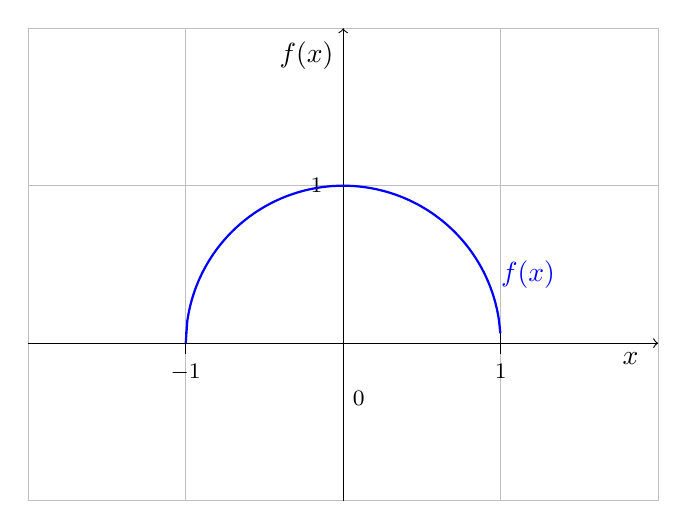
\begin{tikzpicture}[xscale=2, yscale=2]
	
	% Gitternetzlinien
	\draw[xstep=1cm, ystep=1cm, very thin, color=lightgray] (-2,2) grid (2,-1);
	% x-Achse
	\draw[->] (-2,0) -- (2,0) node[below,xshift=-1em] {$x$}; 
	%Zahlen auf x-Achse
	\foreach \x in {-1,...,-1}
	\draw[shift={(\x,0)},color=black] (0pt,2pt) -- (0pt,-2pt) node[below] {\footnotesize $\x$};
	\foreach \x in {1,...,1}
	\draw[shift={(\x,0)},color=black] (0pt,2pt) -- (0pt,-2pt) node[below] {\footnotesize $\x$};
	% y-Achse 
	\draw[->] (0,-1) -- (0,2) node[left,yshift=-1em] {$f(x)$};%node[above left]
	%Zahlen auf y-Achse
	%\foreach \y in {-1,...,-1}
	%\draw[shift={(0,\y)},color=black] (2pt,0pt) -- (-2pt,0pt) node[left] {\footnotesize $\y$};
	\foreach \y in {1,...,1}
	\draw[shift={(0,\y)},color=black] (2pt,0pt) -- (-2pt,0pt) node[left] {\footnotesize $\y$};
	%Ursprung
	\draw[color=black] (0pt,-10pt) node[right] {\footnotesize $0$};
	
	
	
	\draw[thick,color=blue] plot[samples=200, domain=-1:1] 
	(\x,{sqrt(1-\x*\x)}) node[below,yshift=3em,xshift=1em]{$f(x)$};
	
	
	
	\end{tikzpicture}\\
\end{center}
\subsubsection{Trick 6 zur Substitutionsregel}
\href{https://youtu.be/b8ivYOZW2XE}{Video 26}\\
Berechne:\\
\begin{align*}
\int\limits_{}^{} \frac{1}{(x^2+1)^2}\cdot \mathrm{d}x
\end{align*}
Substitution:\\
\begin{align*}
x&=\tan(t)\\
\frac{\mathrm{d}x}{\mathrm{d}t}&=\frac{\mathrm{d}(\tan(t))}{\mathrm{d}t}=1+\tan^2(t)\\
\mathrm{d}x&=(1+\tan^2(t))\mathrm{d}t
\end{align*}
Dann erhält man:\\
\begin{align*}
&=\int\limits_{}^{} \frac{1}{(1+\tan^2(t)+1)^2}\cdot (1+\tan^2(t))\mathrm{d}t\\
&=\int\limits_{}^{} \frac{1}{\tan^2(t)+1}\mathrm{d}t\\
&=\int\limits_{1}^{}\frac{1}{\frac{\sin^2(t)}{\cos^2(t)}+1}\mathrm{d}t \\
&=\int\limits_{}^{} \frac{1}{\frac{\sin^2(t)+\cos^2(t)}{\cos^2(t)}}\mathrm{d}t\\
&=\int\limits_{}^{} \frac{\cos^2(t)}{\sin^2(t)+\cos^2(t)}\mathrm{d}t\\
&=\int\limits_{}^{} \cos^2(t)\mathrm{d}t
\end{align*}
Es gilt mit dem Additionstheorem:\\
\begin{align*}
\cos (2t)&=\cos^2(t)-\sin^2(t)\;\;\;\;\;\;\;\;\;\;\lvert \text{ \tiny +1}\\
\cos (2t)+1&=\cos^2(t)-\sin^2(t)+1\;\;\;\;\lvert \text{\tiny$ \sin^2(t)+\cos^2 (t)=1 $ }\\
\cos (2t)+1&=\cos^2(t)-\sin^2(t)+\sin^2(t)+\cos^2 (t)\\
\cos (2t)+1&=2\cos^2(t)\\
\frac{\cos(2t)+1}{2}&=\cos^2(t)
\end{align*}
Dann ergibt sich:\\
\begin{align*}
&=\int\limits_{}^{} \frac{\cos(2t)+1}{2}\cdot \mathrm{d}t\\
&=\frac{1}{2}\bigg(\frac{1}{2}\sin(2t)+t\bigg)+\alpha,\;\; \alpha\in\mathbb{R}\\
&=\frac{\sin(2t)}{4}+\frac{t}{2}+\alpha,\;\; \alpha\in\mathbb{R}\\
\end{align*}
Rücksubstitution:\\
Es gilt:\\
\begin{align*}
x&=\tan(t)\\
\Leftrightarrow&t=\arctan(x)
\end{align*}
Eingesetzt ergibt sich dann:\\
\begin{align*}
=\frac{\sin(2\arctan(x))}{4}+\frac{\arctan(x)}{2}+\alpha,\;\;\;\;\alpha\in\mathbb{R}
\end{align*}
\subsection{Integration komplexer Funktionen}
\subsubsection{Integration komplexer Funktionen}
\href{https://youtu.be/ms9HZdijOKI}{Video 27}\\
Sei $ f:\mathbb{R}\supset[a,b ] \longmapsto \mathbb{C}$ eine Funktion mit reellem Argument.\\
Dann gilt:\\
\begin{align*}
f(x)=u(x)+\mathrm{i}v(x)\;\;\text{mit }\;\;u,v:[a,b]\longmapsto \mathbb{R}
\end{align*}
Damit definieren wir:\\
\begin{align*}
\int\limits_{a}^{b} f(x)\mathrm{d}x=\int\limits_{a}^{b}u(x) \mathrm{d}x+\mathrm{i}\int\limits_{a}^{b} v(x)\mathrm{d}x
\end{align*}
Somit bleiben alle Integrationsregeln gültig.\\
Beispiel:\\
\begin{align*}
f(x)=x^2+\mathrm{i}x+2=x^2+2+\mathrm{i}x\\
\end{align*}
Das Integral ist dann:\\
\begin{align*}
\int\limits_{}^{} f(x)\mathrm{d}x=\int\limits_{}^{} (x^2+2)\mathrm{d}x+\mathrm{i}\int\limits_{}^{} x\mathrm{d}x=\frac{x^3}{3}+2x+\mathrm{i}\frac{x^2}{2}+\alpha,\;\;\alpha\in \mathbb{C}
\end{align*}
\subsubsection{Aufgabe zur Integration komplexer Funktionen}
\href{https://youtu.be/jG6L4TwLSK0}{Video 28}\\
Berechne:\\
(i)\;\;\;$ \int\limits_{}^{} \frac{1}{(x-\mathrm{i})^2}\cdot \mathrm{d}x $\\
(ii)\;\;$ \int\limits_{}^{} \frac{1}{x-\mathrm{i}}\cdot \mathrm{d}x $\\
Zu (i):\\
\begin{align*}
&\int\limits_{}^{} \frac{1}{(x-\mathrm{i})^2}\cdot \mathrm{d}x=\int\limits_{}^{} (x-1)^{-2}\cdot\mathrm{d}x\\
&\text{Wird wie im reellen Bereich integriert. }
\end{align*}
Zu (ii):\\
\begin{align*}
\int\limits_{}^{} \frac{1}{x-\mathrm{i}}\cdot \mathrm{d}x&=\int\limits_{}^{} \bigg(\frac{x+\mathrm{i}}{x+1}\cdot \frac{1}{x-1}\bigg)\mathrm{d}x\\
&=\int\limits_{}^{}\bigg( \frac{x+\mathrm{i}}{x^2+1}\bigg)\mathrm{d}x\\
&=\int\limits_{}^{} \frac{x}{x^2+1}\cdot \mathrm{d}x+\mathrm{i}\int\limits_{}^{} \frac{1}{x^2+1}\cdot \mathrm{d}x
\end{align*}
Es gilt:\\
\begin{align*}
(\arctan(x))'=\frac{1}{x^2+1}
\end{align*}
Die Ableitung von :\\
\begin{align*}
\big(\ln(x^2+1)\big)'= \frac{2x}{x^2+1}
\end{align*}
Dann ist die Ableitung von:\\
\begin{align*}
\bigg(\frac{1}{2}\ln(x^2+1)\bigg)'=\frac{x}{x^2+1}
\end{align*}
So ergibt sich die Stammfunktion:\\
\begin{align*}
\int\limits_{}^{} \frac{1}{x-\mathrm{i}}\cdot \mathrm{d}x=\frac{1}{2}\ln(x^2+1)+\arctan(x)+\alpha,\;\;\alpha\in \mathbb{C}
\end{align*}
Bemerkung:\\
Die Stammfunktion von $ \int\limits_{}^{} \frac{1}{x-1} \cdot \mathrm{d}x=\ln(x-1)+\alpha$ ist nicht identisch mit der Stammfunktion von $ \int\limits_{}^{} \frac{1}{x-\mathrm{i}} $.\\
\subsection{Integration rationaler Funktionen}
\subsubsection{ Integration rationaler Funktionen/Integration mittels Partialbruchzerlegung}
\href{https://youtu.be/QJQBrXdNNSA}{Video 29}\\
Integration mittels Partialbruchzerlegung (PBZ).
Betrachte:\\
\begin{align*}
\int\limits_{}^{} \frac{x}{x^2-1}\cdot \mathrm{d}x
\end{align*}
\underline{PBZ:}\\
\begin{align*}
(x^2-1)=(x-1)(x+1)
\end{align*}
Es gilt:\\
\begin{align*}
\frac{x}{(x-1)(x+1)}=\frac{\mathrm{A}}{x+1}+\frac{\mathrm{B}}{x-1}
\end{align*}
Bestimmung von A und B mittels Zuhaltemethode:\\
Bemerkung zur Zuhaltemethode: (siehe Skript 7.4.5)\\
Zur Bestimmung von A die Gleichung mit $ (x+1) $ multiplizieren.\\
\begin{align*}
\frac{x(x+1)}{(x-1)(x+1)}=\frac{\mathrm{A(x+1)}}{x+1}+\frac{\mathrm{B(x+1)}}{x-1}\\
\end{align*}
Für $ x=-1 $ gilt dann:\\
\begin{align*}
\frac{x}{(x-1)}=\frac{-1}{(-1-1)}=A=\frac{1}{2}\\
\end{align*}
Für $ x=1 $ gilt dann:\\
\begin{align*}
\frac{x}{x+1}=\frac{1}{(1+1)}=B=\frac{1}{2}
\end{align*}
Dies ergibt dann:\\
\begin{align*}
\frac{x}{x^2-1}=\frac{1}{2(x+1)}+\frac{1}{2(x-1)}
\end{align*}
Die Stammfunktion kann nun leicht berechnet werden.\\
\begin{align*}
\int\limits_{}^{} \frac{x}{x^2-1}\cdot \mathrm{d}x&=\frac{1}{2}\int\limits_{}^{} \frac{1}{x+1}\cdot \mathrm{d}x+\frac{1}{2}\int\limits_{}^{} \frac{1}{x-1}\cdot \mathrm{d}x\\
&=\frac{1}{2}\ln(x+1)+\frac{1}{2}\ln(x-1)+\alpha,\;\;\alpha\in \mathbb{R}
\end{align*}
Mittels der Substitution kann man auch die Stammfunktion: $ \int\limits_{}^{} \frac{x}{x^2-1}\cdot \mathrm{d}x $ bestimmen:\\
Substitution:\\
\begin{align*}
t&=x^2+1\\
\frac{\mathrm{d}t}{\mathrm{d}x}&=\frac{d(x^2-1)}{\mathrm{d}x}=2x\\
\Leftrightarrow \mathrm{d}x&=\frac{\mathrm{\mathrm{d}}t}{2x}
\end{align*}
Dann erhält man:\\
\begin{align*}
&=\int\limits_{}^{} \frac{x}{t}\cdot \frac{\mathrm{d}t}{2x}\\
&=\frac{1}{2}\int\limits_{}^{} \frac{1}{t}\cdot \mathrm{d}t=\frac{1}{2}\ln(t)+\alpha,\;\;\alpha\in\mathbb{R}
\end{align*}
Rücksubstitution mit $ t=x^2-1 $:\\
\begin{align*}
\int\limits_{}^{} \frac{x}{x^2-1}\cdot \mathrm{d}x&=\frac{1}{2}\ln(x^2-1)+\alpha,\;\;\alpha\in\mathbb{R}\\
&=\frac{1}{2}\ln((x+1)(x-1))+\alpha,\;\;\alpha\in\mathbb{R}\\
&=\frac{1}{2}\ln(x+1)+\frac{1}{2}\ln(x-1)+\alpha,\;\;\alpha\in\mathbb{R}\\
\end{align*}
\subsubsection{Aufgabe Integration rationaler Funktionen/Integration mittels Partialbruchzerlegung }
\href{https://youtu.be/CS1aHixYoYU}{Video 30}\\
Berechne:\
\begin{align*}
\int\limits_{2}^{4} \frac{2}{x(x-1)^2}\cdot \mathrm{d}x
\end{align*}
Konstante ausklammern:\\
\begin{align*}
2\int\limits_{}^{}  \frac{1}{x(x-1)^2}\cdot \mathrm{d}x
\end{align*}
PBZ:\\
\begin{align*}
\frac{1}{x(x-1)^2}=\frac{\mathrm{A}}{x}+\frac{\mathrm{B}}{(x-1)}+\frac{C}{(x-1)^2}
\end{align*}
Bemerkung: B und C wegen doppelter Nullstelle.\\
\\
Bestimmung von A,B und C:\\
\begin{quote}
	A und C mit Zuhaltemethode bestimmen:\\
	\begin{align*}
	&\mathrm{A}=\frac{1}{(0-1)^2}=1\\
	&\mathrm{C}=\frac{1}{1}=1
	\end{align*}
	Bestimmung von B:\\
	Es gilt nun:\\
	\begin{align*}
	\frac{1}{x(x-1)^2}=\frac{\mathrm{1}}{x}+\frac{\mathrm{B}}{(x-1)}+\frac{1}{(x-1)^2}
	\end{align*}
	Gleichung mit $ x(x-1)^2 $ multiplizieren ergibt:.\\
	\begin{align*}
	1&=(x-1)^2+\mathrm{B}x(x-1)+x\\
	&=x^2-2x+1+\mathrm{B}x^2-\mathrm{B}x+x\\
	&=(1+\mathrm{B})x^2-x(2+\mathrm{B}-1)+1\\
	0x^2+0x^2+1&=(1+\mathrm{B})x^2-x(2+\mathrm{B}-1)+1\\
	\end{align*}
	Mit Koeffizientenvergleich ergibt sich:\\
	\begin{align*}
	0=1+B\Leftrightarrow B=-1\\
	\end{align*}
	Es gilt nun:\\
	\begin{align*}
	\frac{1}{x(x-1)^2}=\frac{\mathrm{1}}{x}+\frac{\mathrm{-1}}{(x-1)}+\frac{1}{(x-1)^2}
	\end{align*}
\end{quote}
So ergibt sich ein lösbares Integral:\\
\begin{align*}
2\int\limits_{2}^{4} \frac{1}{x(x-1)^2}\cdot \mathrm{d}x&=2\bigg(\int\limits_{2}^{4}\frac{1}{x}\cdot \mathrm{d}x+\int\limits_{2}^{4} \frac{-1}{x-1}\cdot \mathrm{d}x+\int\limits_{0}^{2}\frac{1}{(x-1)^2}\cdot \mathrm{d}x  \bigg)\\
&=2\bigg(\bigg[\ln(x)\bigg]^4_2-\bigg[\ln(x-1)\bigg]^4_2+\bigg[\frac{-1}{x-1}\bigg]^4_2\bigg)\\
&=\text{....weiter mit dem Taschenrechner }
\end{align*}
\subsection{Uneigentliche Integrale }
\subsubsection{Uneigentliche Integrale Teil 1}
\href{https://youtu.be/RO8cL5MA2Bo}{Video 31}\\
Sei $ f:[a,\infty[ \longmapsto \mathbb{R}$ eine Funktion und für jedes Intervall $ [a,b] $ integrierbar.\\
Dann gilt:\\
\begin{align*}
\int\limits_{a}^{\infty} f(x) \mathrm{d}x:=\lim\limits_ {b\to\infty}\int\limits_{a}^{b} f(x)\mathrm{d}x
\end{align*}
$\bullet\;\; \int\limits_{0}^{\infty}=1\mathrm{d}x=\infty $\\
\begin{center}
	
	
	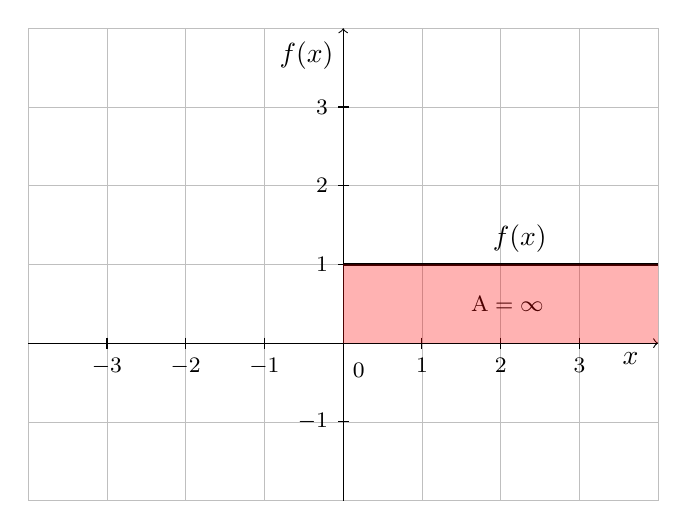
\begin{tikzpicture}[xscale=1, yscale=1]
	
	% Gitternetzlinien
	\draw[xstep=1cm, ystep=1cm, very thin, color=lightgray] (-4,4) grid (4,-2);
	% x-Achse
	\draw[->] (-4,0) -- (4,0) node[below,xshift=-1em] {$x$}; 
	%Zahlen auf x-Achse
	\foreach \x in {-3,...,-1}
	\draw[shift={(\x,0)},color=black] (0pt,2pt) -- (0pt,-2pt) node[below] {\footnotesize $\x$};
	\foreach \x in {1,...,3}
	\draw[shift={(\x,0)},color=black] (0pt,2pt) -- (0pt,-2pt) node[below] {\footnotesize $\x$};
	% y-Achse 
	\draw[->] (0,-2) -- (0,4) node[left,yshift=-1em] {$f(x)$};%node[above left]
	%Zahlen auf y-Achse
	\foreach \y in {-1,...,-1}
	\draw[shift={(0,\y)},color=black] (2pt,0pt) -- (-2pt,0pt) node[left] {\footnotesize $\y$};
	\foreach \y in {1,...,3}
	\draw[shift={(0,\y)},color=black] (2pt,0pt) -- (-2pt,0pt) node[left] {\footnotesize $\y$};
	%Ursprung
	\draw[color=black] (0pt,-10pt) node[right] {\footnotesize $0$};
	
	\draw[thick,color=black] plot[samples=200, domain=0:4] 
	(\x,{1}) node[below, xshift=-5em,yshift=18] {$f(x)$};
	\draw[color=black] (1.5,0.5) node[right] {\footnotesize $\mathrm{A}=\infty$};
	\fill[color =red,fill opacity=0.3] plot[domain=0:4] (\x,{1 })% 
	-- plot[domain=4:0] (\x,{0});% 
	
	
	
	\end{tikzpicture}\\
\end{center}
$ \bullet \;\;\int\limits_{a}^{\infty}\mathrm{e}^x\cdot \mathrm{d}x  $\\

\begin{align*}
\int\limits_{0}^{\infty} \mathrm{e}^{-x}&=\lim\limits_ {b\to\infty}\int\limits_{0}^{b} \mathrm{e}^{-x}\\
&=\lim\limits_ {b\to\infty}\bigg[-\mathrm{e}^{-x}\bigg]^b_0\\
&=\lim\limits_ {b\to\infty}\bigg(-\mathrm{e}^{-b}-(-\mathrm{e}^{-0})\bigg)\\
&=\lim\limits_ {b\to\infty}-\mathrm{e}^{-b}+1\\
&=\lim\limits_ {b\to\infty}\frac{-1}{\mathrm{e}^b}+1=0+1=1
\end{align*}
\begin{center}
	
	
	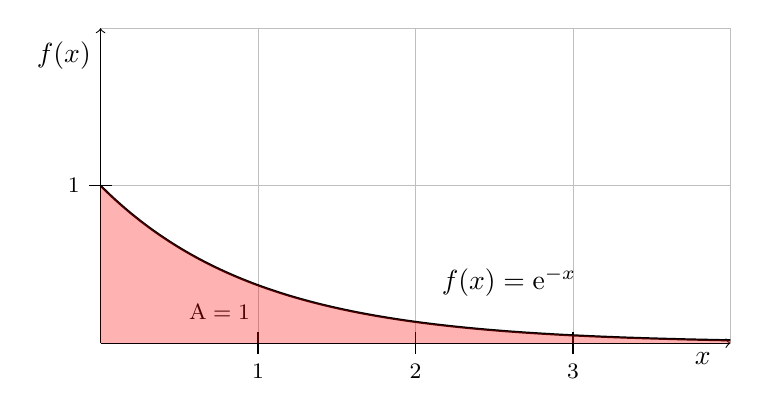
\begin{tikzpicture}[xscale=2, yscale=2]
	
	% Gitternetzlinien
	\draw[xstep=1cm, ystep=1cm, very thin, color=lightgray] (0,2) grid (4,0);
	% x-Achse
	\draw[->] (0,0) -- (4,0) node[below,xshift=-1em] {$x$}; 
	%Zahlen auf x-Achse
	%\foreach \x in {-1,...,-1}
	%\draw[shift={(\x,0)},color=black] (0pt,2pt) -- (0pt,-2pt) node[below] {\footnotesize $\x$};
	\foreach \x in {1,...,3}
	\draw[shift={(\x,0)},color=black] (0pt,2pt) -- (0pt,-2pt) node[below] {\footnotesize $\x$};
	% y-Achse 
	\draw[->] (0,0) -- (0,2) node[left,yshift=-1em] {$f(x)$};%node[above left]
	%Zahlen auf y-Achse
	%\foreach \y in {0,...,-1}
	%\draw[shift={(0,\y)},color=black] (2pt,0pt) -- (-2pt,0pt) node[left] {\footnotesize $\y$};
	\foreach \y in {1,...,1}
	\draw[shift={(0,\y)},color=black] (2pt,0pt) -- (-2pt,0pt) node[left] {\footnotesize $\y$};
	%Ursprung
	%\draw[color=black] (0pt,-10pt) node[right] {\footnotesize $0$};
	
	\draw[thick,color=black] plot[samples=200, domain=0:4] 
	(\x,{e^(-\x)}) node[below, xshift=-8em,yshift=30] {$f(x)=\mathrm{e}^{-x}$};
	\draw[color=black] (.5,0.2) node[right] {\footnotesize $\mathrm{A}=1$};
	\fill[color =red,fill opacity=0.3] plot[domain=0:4] (\x,{e^(-\x) })% 
	-- plot[domain=4:0] (\x,{0});% 
	
	
	
	\end{tikzpicture}\\
\end{center}
Ebenso gilt auch analog für $ f:\;\;]\infty,a]\longmapsto \mathbb{R} $:\\
\begin{align*}
\int\limits_{-\infty}^{a}f(x)\mathrm{d}x =\lim\limits_ {b\to\infty}\int\limits_{b}^{a} f(x)\mathrm{d}x
\end{align*}
\subsubsection{Beispiel zu uneigentlichen Integralen Teil 1}
\href{https://youtu.be/GQxkZxjBx88}{Video 32}\\
Bestimme die Integrale:\\
$ \bullet\;\; \int\limits_{1}^{\infty} \frac{1}{\sqrt{x}}\cdot \mathrm{d}x $\\
\begin{align*}
\int\limits_{1}^{\infty} \frac{1}{\sqrt{x}}\cdot \mathrm{d}x&=\int\limits_{0}^{\infty}x^{-\frac{1}{2}} \cdot \mathrm{d}x\\
&=\lim\limits_ {b\to \infty}\int\limits_{1}^{b} x^{-\frac{1}{2}}\cdot \mathrm{d}x\\
&=\lim\limits_ {b\to\infty}\bigg[2\cdot x^{\frac{1}{2}}\bigg]^b_1\\
&=\lim\limits_ {b\to\infty}(2\sqrt{b}-2)=\infty
\end{align*}
$ \bullet\;\; \int\limits_{1}^{\infty} \frac{1}{x}\cdot \mathrm{d}x $\\
\begin{align*}
\int\limits_{1}^{\infty} \frac{1}{x}\cdot \mathrm{d}x&=\lim\limits_ {b\to\infty}\int\limits_{1}^{b} \frac{1}{x}\cdot \mathrm{d}x\\
&=\lim\limits_ {b\to\infty}\bigg[\ln(x)\bigg]^b_1\\
&=\lim\limits_ {b\to\infty}\big(\ln(b)-\ln(1)\big)=\lim\limits_ {b\to\infty}\ln(b)=\infty
\end{align*}
\begin{center}
	
	
	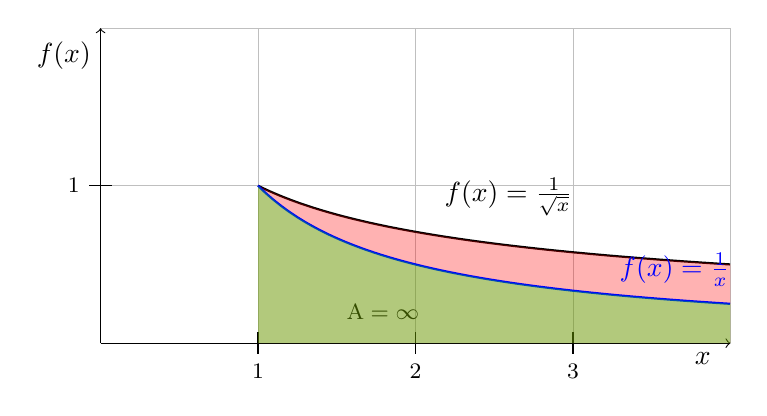
\begin{tikzpicture}[xscale=2, yscale=2]
	
	% Gitternetzlinien
	\draw[xstep=1cm, ystep=1cm, very thin, color=lightgray] (0,2) grid (4,0);
	% x-Achse
	\draw[->] (0,0) -- (4,0) node[below,xshift=-1em] {$x$}; 
	%Zahlen auf x-Achse
	%\foreach \x in {-1,...,-1}
	%\draw[shift={(\x,0)},color=black] (0pt,2pt) -- (0pt,-2pt) node[below] {\footnotesize $\x$};
	\foreach \x in {1,...,3}
	\draw[shift={(\x,0)},color=black] (0pt,2pt) -- (0pt,-2pt) node[below] {\footnotesize $\x$};
	% y-Achse 
	\draw[->] (0,0) -- (0,2) node[left,yshift=-1em] {$f(x)$};%node[above left]
	%Zahlen auf y-Achse
	%\foreach \y in {0,...,-1}
	%\draw[shift={(0,\y)},color=black] (2pt,0pt) -- (-2pt,0pt) node[left] {\footnotesize $\y$};
	\foreach \y in {1,...,1}
	\draw[shift={(0,\y)},color=black] (2pt,0pt) -- (-2pt,0pt) node[left] {\footnotesize $\y$};
	%Ursprung
	%\draw[color=black] (0pt,-10pt) node[right] {\footnotesize $0$};
	
	\draw[thick,color=black] plot[samples=200, domain=1:4] 
	(\x,{1/sqrt(\x)}) node[below, xshift=-8em,yshift=35] {$f(x)=\frac{1}{\sqrt{x}}$};
	\draw[color=black] (1.5,0.2) node[right] {\footnotesize $\mathrm{A}=\infty$};
	\fill[color =red,fill opacity=0.3] plot[domain=1:4] (\x,{1/sqrt(\x) })% 
	-- plot[domain=4:1] (\x,{0});% 
	
	\draw[thick,color=blue] plot[samples=200, domain=1:4] 
	(\x,{1/\x}) node[below, xshift=-2em,yshift=22] {$f(x)=\frac{1}{x}$};
	%\draw[color=blue] (.5,0.2) node[right] {\footnotesize $\mathrm{A}=1$};
	\fill[color =green,fill opacity=0.3] plot[domain=1:4] (\x,{1/\x })% 
	-- plot[domain=4:1] (\x,{0});% 
	
	\end{tikzpicture}\\
\end{center}
$ \bullet\;\; \int\limits_{1}^{\infty} \frac{1}{\sqrt{x^3}}\cdot \mathrm{d}x $\\
\begin{align*}
\int\limits_{1}^{\infty} \frac{1}{\sqrt{x^3}}\cdot \mathrm{d}x&=\lim\limits_ {b\to\infty}x^{-\frac{3}{2}}\cdot \mathrm{d}x\\
&=\lim\limits_ {b\to\infty}\bigg[-2x^{-\frac{1}{2}}\bigg]^b_1\\
&=\lim\limits_ {b\to\infty}\bigg(-\frac{2}{\sqrt{b}}-(-2)\bigg)\\
&=\lim\limits_ {b\to\infty}\bigg(\underbrace {\frac{-2}{\sqrt{b}}}_{\mapsto 0}+2\bigg)=2
\end{align*}
Wenn die Kurve noch steiler wird, wird der Flächeninhalt=2.\\
\begin{center}
	
	
	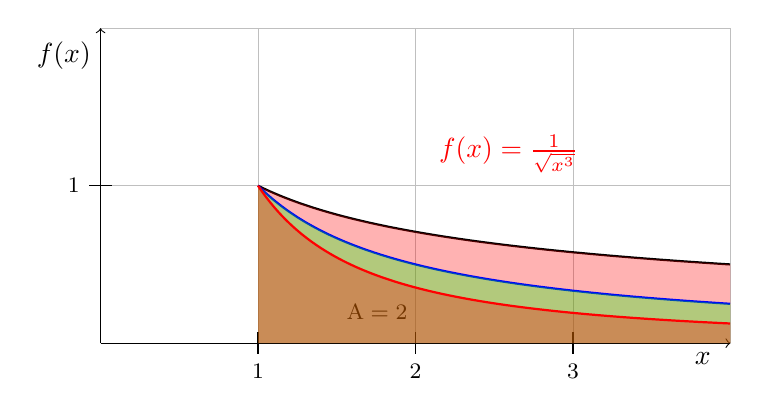
\begin{tikzpicture}[xscale=2, yscale=2]
	
	% Gitternetzlinien
	\draw[xstep=1cm, ystep=1cm, very thin, color=lightgray] (0,2) grid (4,0);
	% x-Achse
	\draw[->] (0,0) -- (4,0) node[below,xshift=-1em] {$x$}; 
	%Zahlen auf x-Achse
	%\foreach \x in {-1,...,-1}
	%\draw[shift={(\x,0)},color=black] (0pt,2pt) -- (0pt,-2pt) node[below] {\footnotesize $\x$};
	\foreach \x in {1,...,3}
	\draw[shift={(\x,0)},color=black] (0pt,2pt) -- (0pt,-2pt) node[below] {\footnotesize $\x$};
	% y-Achse 
	\draw[->] (0,0) -- (0,2) node[left,yshift=-1em] {$f(x)$};%node[above left]
	%Zahlen auf y-Achse
	%\foreach \y in {0,...,-1}
	%\draw[shift={(0,\y)},color=black] (2pt,0pt) -- (-2pt,0pt) node[left] {\footnotesize $\y$};
	\foreach \y in {1,...,1}
	\draw[shift={(0,\y)},color=black] (2pt,0pt) -- (-2pt,0pt) node[left] {\footnotesize $\y$};
	%Ursprung
	%\draw[color=black] (0pt,-10pt) node[right] {\footnotesize $0$};
	
	\draw[thick,color=black] plot[samples=200, domain=1:4] 
	(\x,{1/sqrt(\x)});
	\draw[color=black] (1.5,0.2) node[right] {\footnotesize $\mathrm{A}=2$};
	\fill[color =red,fill opacity=0.3] plot[domain=1:4] (\x,{1/sqrt(\x) })% 
	-- plot[domain=4:1] (\x,{0});% 
	
	\draw[thick,color=blue] plot[samples=200, domain=1:4] 
	(\x,{1/\x});
	%\draw[color=blue] (.5,0.2) node[right] {\footnotesize $\mathrm{A}=1$};
	\fill[color =green,fill opacity=0.3] plot[domain=1:4] (\x,{1/\x })% 
	-- plot[domain=4:1] (\x,{0});% 
	
	\draw[thick,color=red] plot[samples=200, domain=1:4] 
	(\x,{1/sqrt(\x^3)}) node[below, xshift=-8em,yshift=72] {$f(x)=\frac{1}{\sqrt{x^3}}$};
	%\draw[color=blue] (.5,0.2) node[right] {\footnotesize $\mathrm{A}=1$};
	\fill[color =red,fill opacity=0.3] plot[domain=1:4] (\x,{1/sqrt(\x^3) })% 
	-- plot[domain=4:1] (\x,{0});% 
	\end{tikzpicture}\\
\end{center}
\subsubsection{Uneigentliche Integrale Teil 2}
\href{https://youtu.be/ObwW-BSHLz4}{Video 33}\\
Sei $ f:\;]a,b ]$ eine Funktion und existieren für alle $ c\in ]a,b ] $ das $ \int\limits_{c}^{b}f(x) \mathrm{d}x $. Wobei bei $ a $ eine kritische Stelle, wie z.B eine Polstelle ist. \\
Dann definieren wir:\\
\begin{align*}
\int\limits_{a}^{b} f(x)\mathrm{d}x:=\lim\limits_ {\substack{t\mapsto a\\t>a}}\int\limits_{t}^{b} f(x)\mathrm{d}x
\end{align*}
\begin{center}
	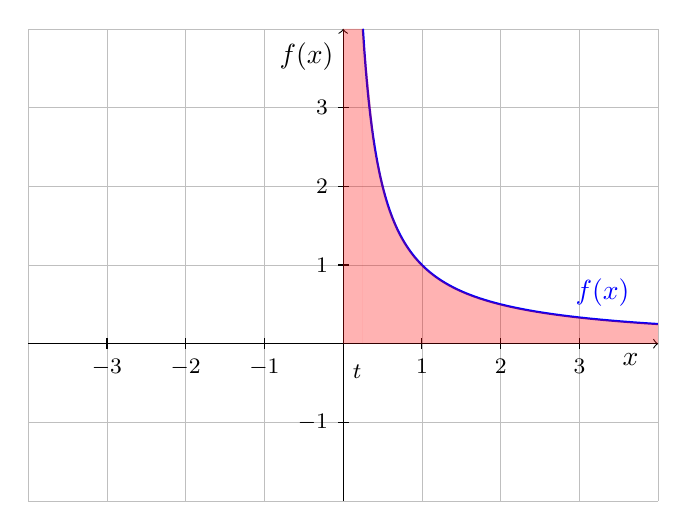
\begin{tikzpicture}[xscale=1, yscale=1]
	
	% Gitternetzlinien
	\draw[xstep=1cm, ystep=1cm, very thin, color=lightgray] (-4,4) grid (4,-2);
	% x-Achse
	\draw[->] (-4,0) -- (4,0) node[below,xshift=-1em] {$x$}; 
	%Zahlen auf x-Achse
	\foreach \x in {-3,...,-1}
	\draw[shift={(\x,0)},color=black] (0pt,2pt) -- (0pt,-2pt) node[below] {\footnotesize $\x$};
	\foreach \x in {1,...,3}
	\draw[shift={(\x,0)},color=black] (0pt,2pt) -- (0pt,-2pt) node[below] {\footnotesize $\x$};
	% y-Achse 
	\draw[->] (0,-2) -- (0,4) node[left,yshift=-1em] {$f(x)$};%node[above left]
	%Zahlen auf y-Achse
	\foreach \y in {-1,...,-1}
	\draw[shift={(0,\y)},color=black] (2pt,0pt) -- (-2pt,0pt) node[left] {\footnotesize $\y$};
	\foreach \y in {1,...,3}
	\draw[shift={(0,\y)},color=black] (2pt,0pt) -- (-2pt,0pt) node[left] {\footnotesize $\y$};
	%Ursprung
	\draw[color=black] (0pt,-10pt) node[right] {\footnotesize $ t$};
	
	\draw[thick,color=blue] plot[samples=200, domain=0.25:4] 
	(\x,{1/\x}) node[below, xshift=-2em,yshift=2em]{$f(x)$};
	
	\fill[color =red,fill opacity=0.3] plot[domain=0.25:4] (\x,{1/\x) })% 
	-- plot[domain=4:0.25] (\x,{0});% 
	\fill[color =red,fill opacity=0.3] plot[domain=0:0.25] (\x,{4 })% 
	-- plot[domain=0.25:0] (\x,{0});% 
	
	
	\end{tikzpicture}\\
\end{center}
Analog definieren wie für $ f:[a, b[ $ das Folgende:\\
\begin{align*}
\int\limits_{a}^{b} f(x)\mathrm{d}x:=\lim\limits_ {\substack{t\mapsto b\\t<b}}\int\limits_{a}^{t} f(x)\mathrm{d}x
\end{align*}
\begin{center}
	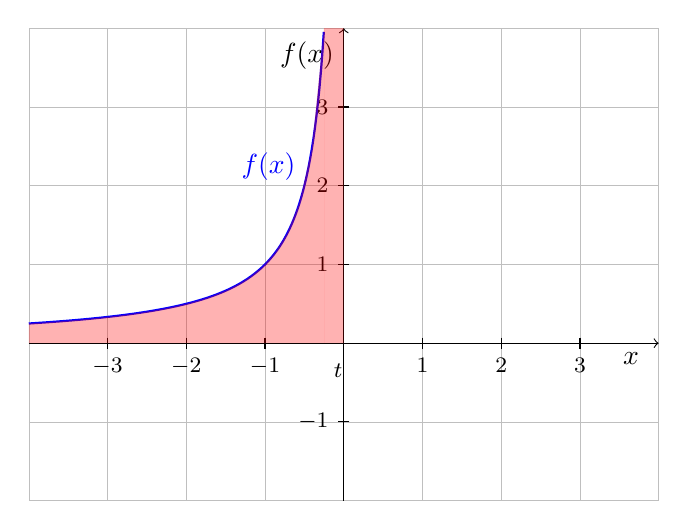
\begin{tikzpicture}[xscale=1, yscale=1]
	
	% Gitternetzlinien
	\draw[xstep=1cm, ystep=1cm, very thin, color=lightgray] (-4,4) grid (4,-2);
	% x-Achse
	\draw[->] (-4,0) -- (4,0) node[below,xshift=-1em] {$x$}; 
	%Zahlen auf x-Achse
	\foreach \x in {-3,...,-1}
	\draw[shift={(\x,0)},color=black] (0pt,2pt) -- (0pt,-2pt) node[below] {\footnotesize $\x$};
	\foreach \x in {1,...,3}
	\draw[shift={(\x,0)},color=black] (0pt,2pt) -- (0pt,-2pt) node[below] {\footnotesize $\x$};
	% y-Achse 
	\draw[->] (0,-2) -- (0,4) node[left,yshift=-1em] {$f(x)$};%node[above left]
	%Zahlen auf y-Achse
	\foreach \y in {-1,...,-1}
	\draw[shift={(0,\y)},color=black] (2pt,0pt) -- (-2pt,0pt) node[left] {\footnotesize $\y$};
	\foreach \y in {1,...,3}
	\draw[shift={(0,\y)},color=black] (2pt,0pt) -- (-2pt,0pt) node[left] {\footnotesize $\y$};
	%Ursprung
	\draw[color=black] (-0.25,-10pt) node[right] {\footnotesize $ t$};
	
	\draw[thick,color=blue] plot[samples=200, domain=-4:-0.25] 
	(\x,{1/-\x}) node[below, xshift=-2em,yshift=-4em]{$f(x)$};
	
	\fill[color =red,fill opacity=0.3] plot[domain=-4:-0.25] (\x,{1/-\x) })% 
	-- plot[domain=-0.25:-4] (\x,{0});% 
	\fill[color =red,fill opacity=0.3] plot[domain=-0.25:0] (\x,{4 })% 
	-- plot[domain=0:-0.25] (\x,{0});% 
	\end{tikzpicture}\\
\end{center}
Beispiel:\\
\begin{align*}
\int\limits_{0}^{2} \frac{1}{x^2}\mathrm{d}x&=\lim\limits_ {\substack{t\mapsto 0\\t>0}}\int\limits_{t}^{2} \frac{1}{x^2}\mathrm{d}x\\
&=\lim\limits_ {\substack{t\mapsto 0\\t>0}}\bigg[-\frac{1}{x}\bigg]^2_t\\
&=\lim\limits_ {\substack{t\mapsto 0\\t>0}}\bigg(-\frac{1}{2}+\underbrace {\frac{1}{t}}_{+\infty}\bigg)=\infty
\end{align*}
\subsubsection{Aufgabe zu uneigentlichen Integralen Teil 2}
\href{https://youtu.be/mUNTuWgMLKA}{Video 34}\\
Für welches $ \alpha \in \;]0,\infty]$ existiert das Integral: $ \int\limits_{0}^{1}\frac{1}{x^\alpha}\mathrm{d}x  $ ?\\
\\
Wie steil muß die Kurve an der Polstelle bei $ x=0 $ werden, dass das Integral existiert und nicht in das Unendliche geht?\\

\begin{align*}
\int\limits_{0}^{1}\frac{1}{x^\alpha} \mathrm{d} x=\lim\limits_{\substack{t\mapsto 0\\t>0}}\int\limits_{t}^{1}\frac{1}{x^\alpha}\mathrm{d}x=\lim\limits_ {\substack{t\mapsto 0\\t>0}} \bigg[\frac{1}{1-\alpha}x^{-\alpha+1}\bigg]^1_t=\lim\limits_ {\substack{t\mapsto 0\\t>0}}\bigg(\frac{1}{1-\alpha}-\frac{1}{1-\alpha}t^{1-\alpha}\bigg)
\end{align*}
Die Frage: Wann wird der $ \lim\limits_ {t\mapsto 0} t^{1-\alpha}$ unendlich oder Null? Für $ 1-\alpha<0 $ ist die Hochzahl negativ $ \Rightarrow \lim\limits_ {t\mapsto 0} \frac{1}{t^\beta}=\infty$ mit $ \beta>0 $ und für $1-\alpha>0  $ ist die Hochzahl positiv $ \Rightarrow \lim\limits_ {t\mapsto 0}t^\beta=0 $ mit $ \beta>0 $.\\
Fallunterscheidung:\\
1. Fall: $ 1-\alpha<0$\\
\begin{quote}
	
	
	\begin{align*}
	\alpha>1\Leftrightarrow 1-\alpha<0
	\end{align*}
	Dann gilt:\\
	\begin{align*}
	&t^{1-\alpha}=t^{-\beta}=\frac{1}{t^\beta} \;\;\text{mit }\beta>0\\
	&\lim\limits_ {t\to 0}\frac{1}{t^\beta}=\infty\\
	&\Rightarrow \int\limits_{0}^{1}\frac{1}{x^\alpha} \mathrm{d} x=\lim\limits_ {\substack{t\mapsto 0\\t>0}}\bigg(\frac{1}{1-\alpha}-\frac{1}{1-\alpha}t^{1-\alpha}\bigg)=\infty
	\end{align*}
	Das Integral geht gegen unendlich für $ \alpha>1 $. Es existiert kein Grenzwert.\\
\end{quote}
2. Fall: $ 1-\alpha>0$\\
\begin{quote}
	\begin{align*}
	\alpha<1\Leftrightarrow 1-\alpha>0
	\end{align*}
	Dann git:\\
	\begin{align*}
	&t^{1-\alpha}=t^\beta \;\;\text{mit }\beta>0\\
	&\lim\limits_ {t\to 0}t^\beta=0\\
	&\Rightarrow \int\limits_{0}^{1}\frac{1}{x^\alpha} \mathrm{d} x=\lim\limits_ {\substack{t\mapsto 0\\t>0}}\bigg(\frac{1}{1-\alpha}-\frac{1}{1-\alpha}t^{1-\alpha}\bigg)=\frac{1}{1-\alpha}
	\end{align*}
	Das Integral geht gegen einen Grenzwert für $ \alpha<1 $. Es existiert ein Grenzwert.\\
\end{quote}
Beispiel:\\
Ein Integral existiert für: $ \alpha=\frac{1}{2} $\\
\begin{align*}
\int\limits_{0}^{1} \frac{1}{\sqrt{x}}\mathrm{d}x
\end{align*}
Es existiert kein Integral für: $ \alpha=2 $\\
\begin{align*}
\int\limits_{0}^{1} \frac{1}{x^2}\mathrm{d}x
\end{align*}
\begin{center}
	
	
	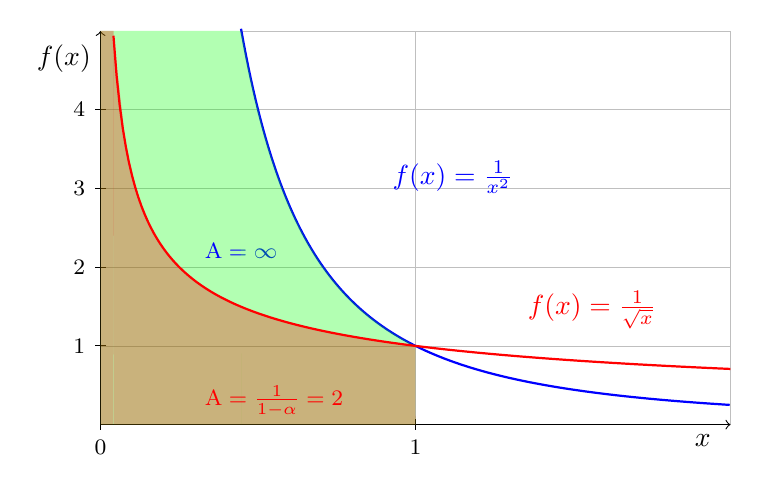
\begin{tikzpicture}[xscale=4, yscale=1]
	
	% Gitternetzlinien
	\draw[xstep=1cm, ystep=1cm, very thin, color=lightgray] (0,5) grid (2,0);
	% x-Achse
	\draw[->] (0,0) -- (2,0) node[below,xshift=-1em] {$x$}; 
	%Zahlen auf x-Achse
	%\foreach \x in {-1,...,-1}
	%\draw[shift={(\x,0)},color=black] (0pt,2pt) -- (0pt,-2pt) node[below] {\footnotesize $\x$};
	\foreach \x in {0,...,1}
	\draw[shift={(\x,0)},color=black] (0pt,2pt) -- (0pt,-2pt) node[below] {\footnotesize $\x$};
	% y-Achse 
	\draw[->] (0,0) -- (0,5) node[left,yshift=-1em] {$f(x)$};%node[above left]
	%Zahlen auf y-Achse
	%\foreach \y in {0,...,-1}
	%\draw[shift={(0,\y)},color=black] (2pt,0pt) -- (-2pt,0pt) node[left] {\footnotesize $\y$};
	\foreach \y in {1,...,4}
	\draw[shift={(0,\y)},color=black] (0.5pt,0pt) -- (-0.5pt,0pt) node[left] {\footnotesize $\y$};
	%Ursprung
	%\draw[color=black] (-1pt,-10pt) node[right] {\footnotesize $0$};
	
	%\draw[thick,color=black] plot[samples=200, domain=0.20:1] 
	%(\x,{1/\x}) node[below, xshift=-8em,yshift=102] {$f(x)=\frac{1}{x }$};
	%\draw[color=black] (1.5,0.2) node[right] {\footnotesize $\mathrm{A}=2$};
	%\fill[color =red,fill opacity=0.3] plot[domain=0.28:4] (\x,{1/\x })% 
	%-- plot[domain=4:0.28] (\x,{0});% 
	\draw[thick,color=white] plot[samples=200, domain=0.:0.446] 
	(\x,{5});
	
	\fill[color =green,fill opacity=0.3] plot[domain=0:0.446] (\x,{5 })% 
	-- plot[domain=0.446:0] (\x,{0});% 
	
	
	\draw[thick,color=blue] plot[samples=200, domain=0.446:2] 
	(\x,{1/\x^2}) node[below, xshift=-10em,yshift=92] {$f(x)=\frac{1}{x^2 }$};
	\draw[color=blue] (.3,2.2) node[right] {\footnotesize $\mathrm{A}=\infty$};
	\fill[color =green,fill opacity=0.3] plot[domain=0.446:1] (\x,{1/\x^2 })% 
	-- plot[domain=1:0.446] (\x,{0});% 
	
	\draw[thick,color=red] plot[samples=200, domain=0.041:2] 
	(\x,{1/(sqrt(\x))}) node[below, xshift=-5em,yshift=32] {$f(x)=\frac{1}{\sqrt{x}}$};
	\draw[color=red] (.3,0.3) node[right] {\footnotesize $\mathrm{A}=\frac{1}{1-\alpha}=2$};
	\fill[color =red,fill opacity=0.3] plot[domain=0.041:1] (\x,{1/(sqrt(\x)) })% 
	-- plot[domain=1:0.041] (\x,{0});% 
	
	
	\fill[color =red,fill opacity=0.3] plot[domain=0:0.042] (\x,{5 })% 
	-- plot[domain=0.041:0] (\x,{0});% 
	\end{tikzpicture}\\
\end{center}
\subsubsection{Majorantenkriterium für uneigentliche }
\href{https://youtu.be/qe4opJMGitY}{Video 35}\\
Seien $ a\in\mathbb{R} $ und $ b\in\mathbb{R}\cup\{\infty\} $ und $ f,g:[a,b[\;\longmapsto \mathbb{R} $ Funktionen, die auf allen Intervallen $ [a,c] $ mit $ a<c<b $ integrierbar sind, dann gilt das Majorantenkriterium.\\
\\
\underline{Majorantenkriterium:}\\
Ist $ \lvert f(x)\lvert\leq g(x) $ für alle $ x\in[a,b[ $ und existiert das Integral: $ \int\limits_{a}^{b}g(x) \mathrm{d}x $, dann existiert auch das Integral: $ \int\limits_{a}^{b}f(x)\mathrm{d}x  $.\\
\begin{center}
	\begin{align*}
	\lvert f(x)\lvert\leq g(x)\;\;\text{für alle }\;\;x\in[-2,2]
	\end{align*}
	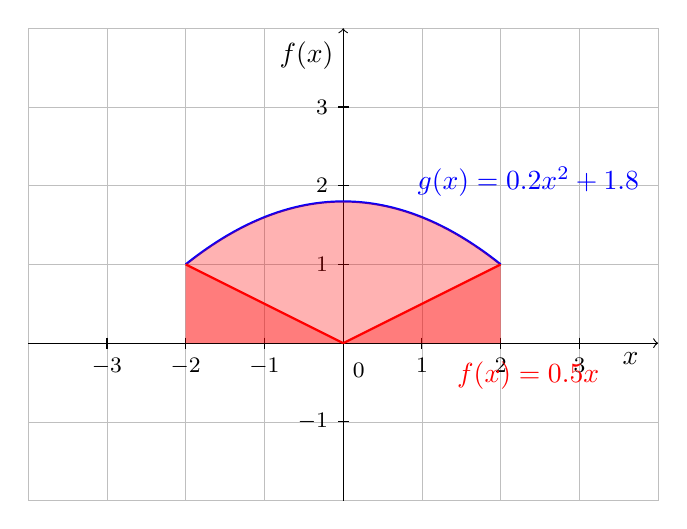
\begin{tikzpicture}[xscale=1, yscale=1]
	
	% Gitternetzlinien
	\draw[xstep=1cm, ystep=1cm, very thin, color=lightgray] (-4,4) grid (4,-2);
	% x-Achse
	\draw[->] (-4,0) -- (4,0) node[below,xshift=-1em] {$x$}; 
	%Zahlen auf x-Achse
	\foreach \x in {-3,...,-1}
	\draw[shift={(\x,0)},color=black] (0pt,2pt) -- (0pt,-2pt) node[below] {\footnotesize $\x$};
	\foreach \x in {1,...,3}
	\draw[shift={(\x,0)},color=black] (0pt,2pt) -- (0pt,-2pt) node[below] {\footnotesize $\x$};
	% y-Achse 
	\draw[->] (0,-2) -- (0,4) node[left,yshift=-1em] {$f(x)$};%node[above left]
	%Zahlen auf y-Achse
	\foreach \y in {-1,...,-1}
	\draw[shift={(0,\y)},color=black] (2pt,0pt) -- (-2pt,0pt) node[left] {\footnotesize $\y$};
	\foreach \y in {1,...,3}
	\draw[shift={(0,\y)},color=black] (2pt,0pt) -- (-2pt,0pt) node[left] {\footnotesize $\y$};
	%Ursprung
	\draw[color=black] (0pt,-10pt) node[right] {\footnotesize $0$};
	
	\draw[thick,color=blue] plot[samples=200, domain=-2:2] 
	(\x,{-\x*\x*0.2+1.8}) node[yshift=3em, xshift=1em] {$g(x)=0.2x^2+1.8$};
	
	\draw[thick,color=red] plot[samples=200, domain=0:2] 
	(\x,{0.5*\x}) node[yshift=-4em, xshift=1em]{$\lvert f(x)\lvert=0.5x $};
	\draw[thick,color=red] plot[samples=200, domain=-2:0] 
	(\x,{-0.5*\x});
	
	\fill[color =red,fill opacity=0.3] plot[domain=-2:0] (\x,{-0.5*\x })% 
	-- plot[domain=0:-2] (\x,{0});% 
	\fill[color =red,fill opacity=0.3] plot[domain=0:2] (\x,{0.5*\x })% 
	-- plot[domain=2:0] (\x,{0});% 
	\fill[color =red,fill opacity=0.3] plot[domain=-2:2] (\x,{-\x*\x*0.2+1.8 })% 
	-- plot[domain=2:-2] (\x,{0});% 
	\end{tikzpicture}\\	
\end{center}
Beispiel:\\
Existiert das Integral:\\
\begin{align*}
\int\limits_{1}^{\infty}\frac{\mathrm{e}^{-x}}{x} \mathrm{d}x
\end{align*}
Sei:\\
\begin{align*}
f(x)=\frac{\mathrm{e}^{-x}}{x}
\end{align*}
dann ist:\\
\begin{align*}
\lvert f(x)\lvert=\frac{\mathrm{e}^{-x}}{x}\leq \mathrm{e}^{-x}
\end{align*}
Betrachte:\\
\begin{align*}
\int\limits_{0}^{\infty} \mathrm{e}^{-x}\mathrm{d}x=\lim\limits_ {b\to\infty}\int\limits_{1}^{b} \mathrm{e}^{-x}\mathrm{d}x=\lim\limits_ {b\to\infty}\bigg[-\mathrm{e}^{-x}\bigg]^b_1&=\lim\limits_ {b\to\infty}\bigg(-\mathrm{e}^{-b}-(-e^{-1})\bigg)\\
&=\lim\limits_ {b\to\infty}\bigg(\underbrace {-\frac{1}{\mathrm{e}^b}}_{\mapsto 0}+\mathrm{e}^{-1}\bigg)=\mathrm{e}^{-1}=\frac{1}{\mathrm{e}}\\
\int\limits_{0}^{\infty} \mathrm{e}^{-x}\mathrm{d}x&=\frac{1}{\mathrm{e}}
\end{align*}
Nach dem Majorantenkriterium gilt:\\
\begin{align*}
\lvert f(x)\lvert\leq g(x) 
\end{align*}
Da die Funktion $ \int\limits_{1}^{\infty} g(x)\mathrm{d}x $ existiert folgt nach dem Majorantenkriterium, dass das Integral:\\
\begin{align*}
\int\limits_{1}^{\infty}\frac{\mathrm{e}^{-x}}{x} \mathrm{d}x
\end{align*}
auch existiert.\\
Bemerkung:\\
Existiert kein Grenzwert, so kann keine Aussage getroffen werden, ob das Integral existiert.\\
Das Integral $ \int\limits_{1}^{\infty}\frac{1}{\sqrt{x^3}} \mathrm{d}x=2 $ und das Integral $ \int\limits_{1}^{\infty} \frac{1}{x} \mathrm{dx}=\infty$.\\
Aber $ |f(x)|=\frac{1}{\sqrt{x^3}}<g(x)=\frac{1}{x} $ im Bereich von $ x\in   [1,\infty[ $ .
\subsubsection{Minorantenkriterium für uneigentliche Integrale}
\href{https://youtu.be/wBYcVF1449w}{Video 36}\\
Seien $ a\in\mathbb{R} $ und $ b\in\mathbb{R}\cup\{\infty\} $ und $ f,g:[a,b[\;\longmapsto \mathbb{R} $ Funktionen, die auf allen Intervallen $ [a,c] $ mit $ a<c<b $ integrierbar sind, dann gilt das Minorantenkriterium.\\
Gelte:\\
\begin{align*}
0\leq g(x) \leq f(x)\;\;\text{für alle } x\in[a,c[
\end{align*}
und existieren nicht:\\
\begin{align*}
\int\limits_{a}^{b} g(x)\mathrm{d}x=\lim\limits_ {\substack{t\mapsto b \\ t<b}}\int\limits_{a}^{b} g(x)\mathrm{d}x
\end{align*}
dann existiert auch nicht:
\begin{align*}
\int\limits_{a}^{b} f(x)\mathrm{d}x
\end{align*}
Mit dem Minorantenkriterium zeigt man, dass kein Grenzwert existiert. Denn wenn die kleinere Funktion $ g(x) $ divergiert, dann divergiert auch $ f(x) $.\\
Mit dem Majorantenkriterium zeigt man, dass eine Konvergenz existiert.\\
\\
Beispiel:\\
Existiert das Integral:\\
\begin{align*}
\int\limits_{1}^{\infty} \cosh(x)\mathrm{d}x
\end{align*}
Es gilt:\\
\begin{align*}
0\leq 1 \leq \cosh(x)
\end{align*}
Bemerkung:\\
\begin{align*}
&\cosh(x)=\frac{e^x+e^{-1}}{2}\\
&x=0\Rightarrow \cosh(x)=1
\end{align*}
Daraus folgt dann:\\
\begin{align*}
&g(x)=1\\
&\int\limits_{1}^{\infty} 1\mathrm{d}x=\lim\limits_ {t\to\infty}\int\limits_{1}^{t} 1\mathrm{d}x=\lim\limits_ {t\to\infty}\bigg[x\bigg]^t_1=\lim\limits_ {t\to\infty} t-1=\infty
\end{align*}
Mit dem Minorantenkriterium gilt dann:\\
\begin{align*}
\int\limits_{1}^{\infty} 1\mathrm{d}x=\int\limits_{1}^{\infty} =\infty\overset{Minorantenkr.}{\longmapsto}\int\limits_{1}^{\infty} \cosh(x)\mathrm{d}x\;\;\text{existiert nicht }
\end{align*}
\subsubsection{Aufgabe 1 zum Minoranten- und Majorantenkriterium für uneigentliche Integrale}
\href{https://youtu.be/xJGJ5_nopx0}{Video 37}\\
Existiert das Integral:\\
\begin{align*}
\int\limits_{0}^{1} \frac{1}{(2+x^3)^{\frac{3}{2}}}\mathrm{d}x
\end{align*}
Betrachte mit dem Majoratenkriterium:\\
\begin{align*}
&\lvert f(x)\lvert\leq g(x) \\
&f(x)=\bigg|\frac{1}{(2+x^3)^{\frac{3}{2}}}\bigg|\\
&\text{für }\\x>0\Rightarrow \text{Betrag fällt weg }
\end{align*}
Abschätzen von $ g(x) $:\\
\begin{align*}
f(x)=\frac{1}{(2+x^3)^{\frac{3}{2}}}\leq \frac{1}{(x^3)^{\frac{3}{2}}}=\frac{1}{x^{\frac{9}{2}}}=x^{-\frac{9}{2}}=g(x)\;\;\text{ für}\;\;x\in[1,\infty[
\end{align*}
Integral von $\int\limits_{1}^{\infty}  g(x)\mathrm{d}x $ berechnen:\\
\begin{align*}
\int\limits_{0}^{\infty} x^{-\frac{9}{2}}\mathrm{d}x=\lim\limits_ {b\to\infty}\int\limits_{1}^{b} x^{-\frac{9}{2}}\mathrm{d}x&=\lim\limits_ {b\to\infty}\bigg[-\frac{2}{7}x^{-\frac{7}{2}}\bigg]^b_1\\
&=\lim\limits_ {b\to\infty}\bigg(-\frac{2}{7}\frac{1}{b^{\frac{7}{2}}}-\big(-\frac{2}{7}\big)\bigg)=\frac{2}{7}\\
&\overset{Majork.}{\Rightarrow}\int\limits_{0}^{\infty} f(x)\mathrm{d}x=\int\limits_{1}^{\infty} \frac{1}{(2+x^3)^{\frac{3}{2}}}\mathrm{d}x\;\;\text{existiert. }
\end{align*}
\subsubsection{Aufgabe 2 zum Minoranten- und Majorantenkriterium für uneigentliche Integrale}
\href{https://youtu.be/XJG5oZmOEVE}{Video 38}\\
Existiert das Integral:\\
\begin{align*}
\int\limits_{2}^{\infty} \frac{2+\cos(x)}{\sqrt{x^2-1}}\mathrm{d}x
\end{align*}
Die Frage:\\
Welches Kriterium verwendet man?\\
Wenn das Interal nicht existiert, dann verwenden wir das Minorantekriterium, sonst das Majorantenkriterium.\\
Durch Abschätzen und Überlegung bekommt man für $ x\in[2,\infty[ $:\\
Der $ \cos(x) $ liegt zwischen -1 und 1. Der Zähler wird nicht größer als 3 und nicht kleiner als 1.\\
$ \sqrt{x^2-1} $ ist kleiner als $ \sqrt{x^2}=x $ daraus folgt dann:\\
\begin{align*}
\frac{2+\cos(x)}{\sqrt{x^2-1}}>\frac{1}{\sqrt{x^2-1}}>\frac{1}{x}
\end{align*}
Nun nehmen wir an, dass kein Integral existiert.\\
Es gilt mit dem Minorantenkriterium:\\
\begin{align*}
0\leq g(x)\leq f(x)
\end{align*}
Es gilt:\\
\begin{align*}
0\leq \frac{1}{x}\leq \frac{2+\cos(x)}{\sqrt{x^2-1}}
\end{align*}
Nun bestimmen wir das Integal: $ \int\limits_{2}^{\infty} g(x)\mathrm{d}x=\int\limits_{2}^{\infty} \frac{1}{x}\mathrm{d}x $\\
\begin{align*}
\int\limits_{2}^{\infty} g(x)=\lim\limits_ {t\to\infty}\int\limits_{2}^{t}\frac{1}{x}\mathrm{d} x=\lim\limits_ {t\to\infty}\bigg[\ln(x)\bigg]^t_2=\lim\limits_ {t\to\infty}\bigg(\ln(t)-\ln(2)\bigg)=\infty
\end{align*}
\begin{align*}
\overset{Minork.}{\Rightarrow}\int\limits_{2}^{\infty} f(x)\mathrm{d}x=\int\limits_{2}^{\infty} \frac{2+\cos(x)}{\sqrt{x^2-1}}\mathrm{d}x\;\;\text{existiert nicht. }
\end{align*}
